\chapter{Implementation and Evaluation}
\label{ch:implementation}

\section{Introduction}

This chapter is, in many ways, where the design decisions of the previous chapter either hold up or fall apart. What was built is a working Progressive Web Application comprising roughly 105 TypeScript source files, three trained machine learning models, and a dual-layer offline data management architecture. Whether it actually works as intended is the question the evaluation half of this chapter answers --- through offline functionality tests, performance measurement, cross-platform compatibility checks, and a structured usability assessment with nine real IPDC stakeholders.

\section{Development Environment and Tools}

\subsection{Development Setup}

The development environment centered on Visual Studio Code as the primary IDE, Node.js (v18+) as the JavaScript runtime, React 19.2.1 \citep{React2024} as the frontend framework, and the Vite development server for hot module replacement at \texttt{localhost:5173}. Firebase emulators handled local testing of authentication and Firestore operations, avoiding unnecessary consumption of cloud quotas. The AI model backend was developed separately in a Python environment using FastAPI, with models available at \texttt{localhost:8000}.

\subsection{Project Structure}

The project follows a modular directory structure organized by concern. Application source code lives in \texttt{src/}, while machine learning components and the API server reside in \texttt{ai-models/}. Table~\ref{tab:project-structure} provides an overview of the directory layout and component counts.

\begin{table}[H]
\centering
\caption{Project Directory Structure and Component Counts}
\label{tab:project-structure}
\small
\begin{tabular}{p{3.8cm}p{7.5cm}l}
\toprule
\textbf{Directory} & \textbf{Purpose} & \textbf{Files} \\
\midrule
src/components/admin/ & Admin-specific UI components & 6 \\
src/components/common/ & Shared UI components (StatusBar, FileUpload, etc.) & 12 \\
src/components/layout/ & Navigation and layout scaffolding & 3 \\
src/components/map/ & Interactive park map and details & 3 \\
src/components/operations/ & Operations module components & 4 \\
src/components/tenant/ & Tenant-specific components & 13 \\
src/pages/ & Page-level route components & 15 \\
src/services/ & Business logic and API services & 18 \\
src/services/offline/ & Offline storage and sync services & 3 \\
src/contexts/ & React context providers & 1 \\
src/hooks/ & Custom React hooks & 4 \\
src/db/ & Dexie.js schema definition & 1 \\
src/types/ & TypeScript type definitions & 8 \\
src/config/ & Firebase and theme configuration & 2 \\
ai-models/ & Three ML models + FastAPI backend & 12 \\
\midrule
\textbf{Total} & & \textbf{$\sim$105} \\
\bottomrule
\end{tabular}
\end{table}

\subsection{Build and Deployment Configuration}

The Vite build uses manual chunk splitting (\texttt{vendor}, \texttt{mui}, \texttt{firebase}) so application updates do not invalidate cached library bundles --- valuable where connectivity is limited.

The vite-plugin-pwa generates the service worker and web app manifest automatically from the configuration in \texttt{vite.config.ts}. The deployed platform is accessible at the following URLs:

\begin{itemize}
  \item \textbf{Frontend Application:} \url{https://ipdc-oss-platform.vercel.app/} --- deployed on Vercel with HTTPS, global CDN distribution, and automatic SSL certificate management.
  \item \textbf{AI Backend API:} \url{https://ipdc-oss-platform.onrender.com/api/docs} --- deployed on Render, hosting the FastAPI server with the three trained ML models. Interactive API documentation (Swagger UI) is available at this URL; model endpoints are served under the \texttt{/api/v1/} prefix (e.g., \texttt{/api/v1/classify-service}, \texttt{/api/v1/predict-maintenance}, \texttt{/api/v1/recommend-parks}).
\end{itemize}

\section{Key Feature Implementation}

\subsection{Offline-First Architecture Implementation}

The offline-first architecture is realized through three cooperating subsystems: Firebase Firestore's transparent cache, the Dexie.js local database, and a custom synchronization service.

\textbf{Firebase Offline Persistence} is activated in the Firebase configuration module (\texttt{src/config/firebase.ts}) during initialization:

\begin{lstlisting}[language=Java, caption={Firebase Offline Persistence Configuration}, label={lst:firebase-config}]
initializeFirestore(app, {
  localCache: persistentLocalCache({
    tabManager: persistentMultipleTabManager()
  })
});
\end{lstlisting}

This instructs Firestore to maintain a persistent local cache of all documents the user has accessed, keeping it intact across browser sessions and coordinating access when multiple tabs are open. When the network is unavailable, reads are served from this cache and writes are internally queued for later synchronization.

\textbf{Dexie.js Local Database} extends Firestore's cache with explicit offline data management. The schema, defined in \texttt{src/db/schema.ts}, sets up two indexed tables:

\begin{lstlisting}[language=Java, caption={Dexie.js Database Schema}, label={lst:dexie-schema}]
const db = new Dexie('IPDCDatabase');
db.version(1).stores({
  serviceRequests:
    'id, tenantId, status, priority, serviceType, createdAt',
  syncQueue:
    '++id, type, collection, status, createdAt'
});
\end{lstlisting}

\textbf{The Sync Service} (\texttt{src/services/offline/syncService.ts}) picks up queued items once connectivity is detected. It iterates through pending entries, converts local JavaScript \texttt{Date} objects to Firestore \texttt{Timestamp} objects, writes to the appropriate collection, and marks each item with an updated status. A built-in retry mechanism handles transient failures so no queued data is lost.

\subsection{Authentication with Offline Fallback}

The authentication system implements the dual-mode design outlined in Chapter~\ref{ch:analysis}. The \texttt{AuthContext} (\texttt{src/contexts/AuthContext.tsx}) wraps the entire application and manages authentication state. When signing in online, credentials are verified through Firebase Auth and cached locally:

\begin{lstlisting}[language=Java, caption={Credential Caching After Online Authentication}, label={lst:auth-cache}]
// After successful Firebase Auth sign-in:
await cacheCredentials(email, password);
await cacheAuthState({
  uid: user.uid,
  email: user.email,
  displayName: user.displayName,
  role: userData.role
});
\end{lstlisting}

If the sign-in attempt fails because of a network error, the context automatically falls back to offline verification:

\begin{lstlisting}[language=Java, caption={Offline Authentication Fallback}, label={lst:auth-offline}]
// Network error detected during sign-in:
const isValid = await verifyOfflineCredentials(email, password);
if (isValid) {
  const cachedUser = await getCachedAuthState();
  // Grant access using cached user profile
}
\end{lstlisting}

Any user who has previously authenticated while online can therefore continue using the platform during connectivity outages. Figure~\ref{fig:auth-interfaces} shows the sign-in and tenant registration interfaces.

\begin{figure}[H]
\centering
\begin{minipage}[t]{0.48\textwidth}
\centering
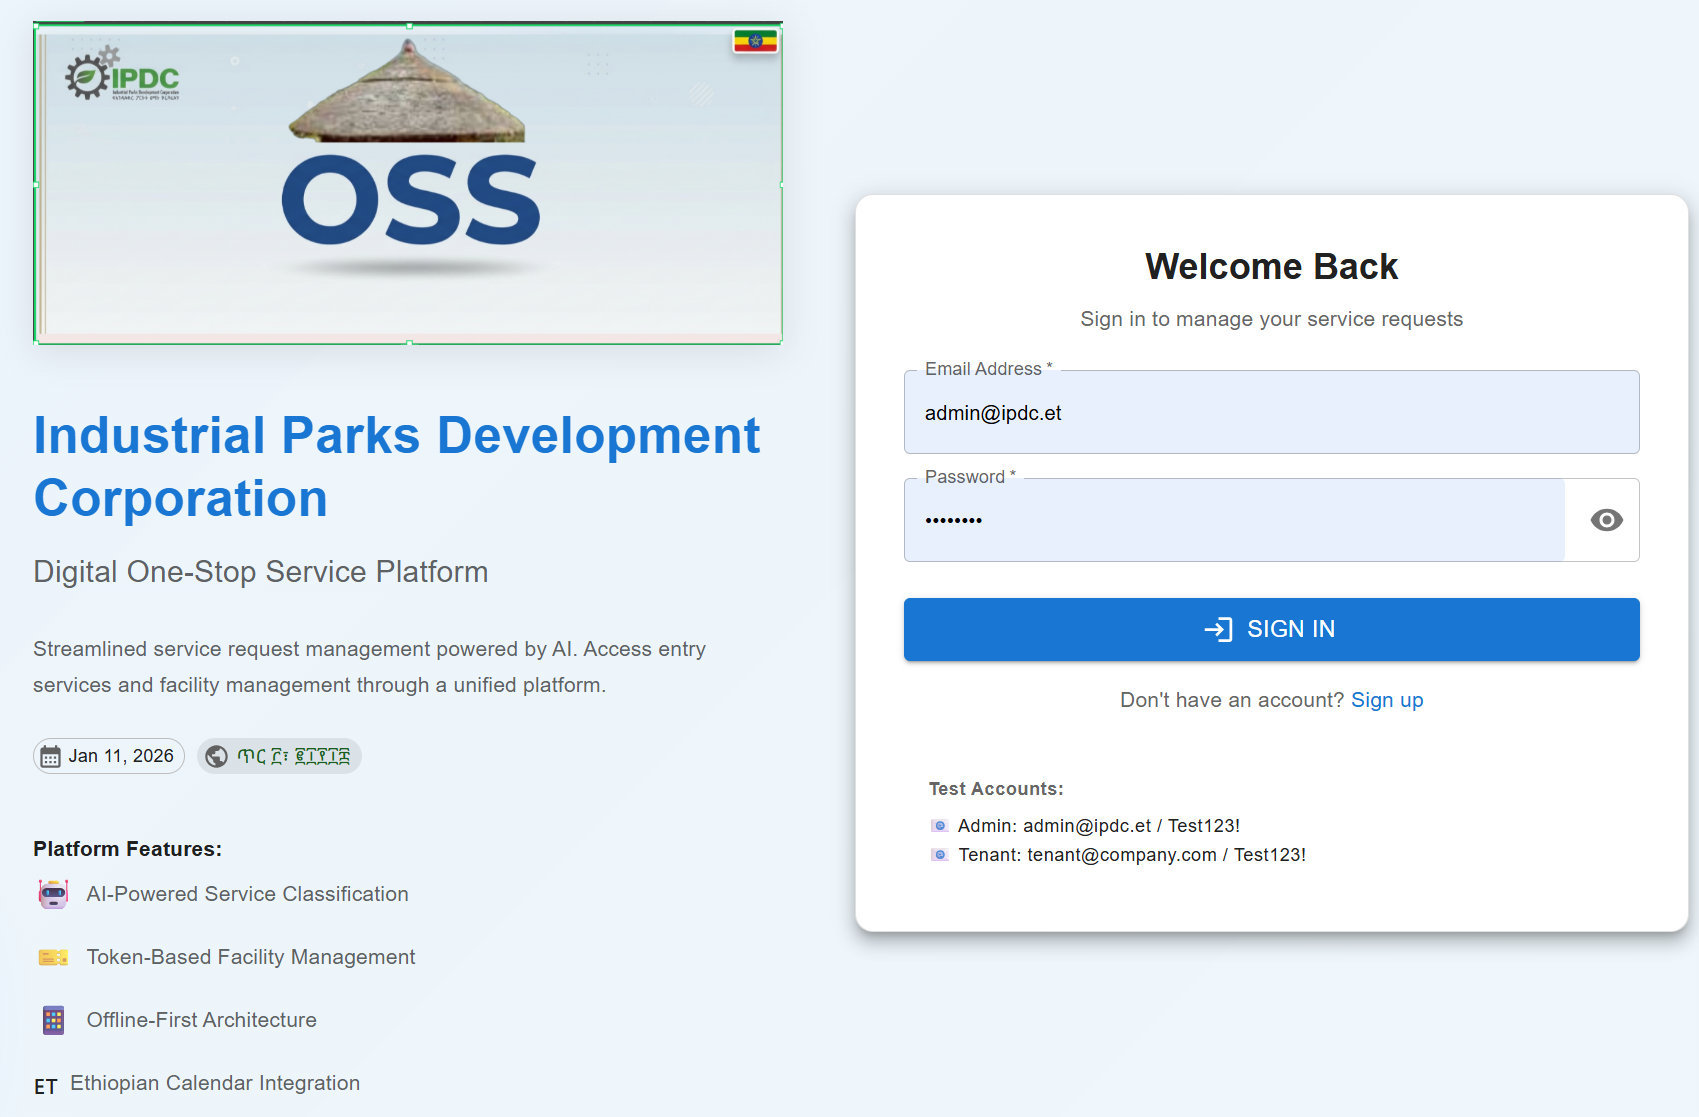
\includegraphics[width=\textwidth]{figures/fig_sign_in.png}
\end{minipage}
\hfill
\begin{minipage}[t]{0.48\textwidth}
\centering
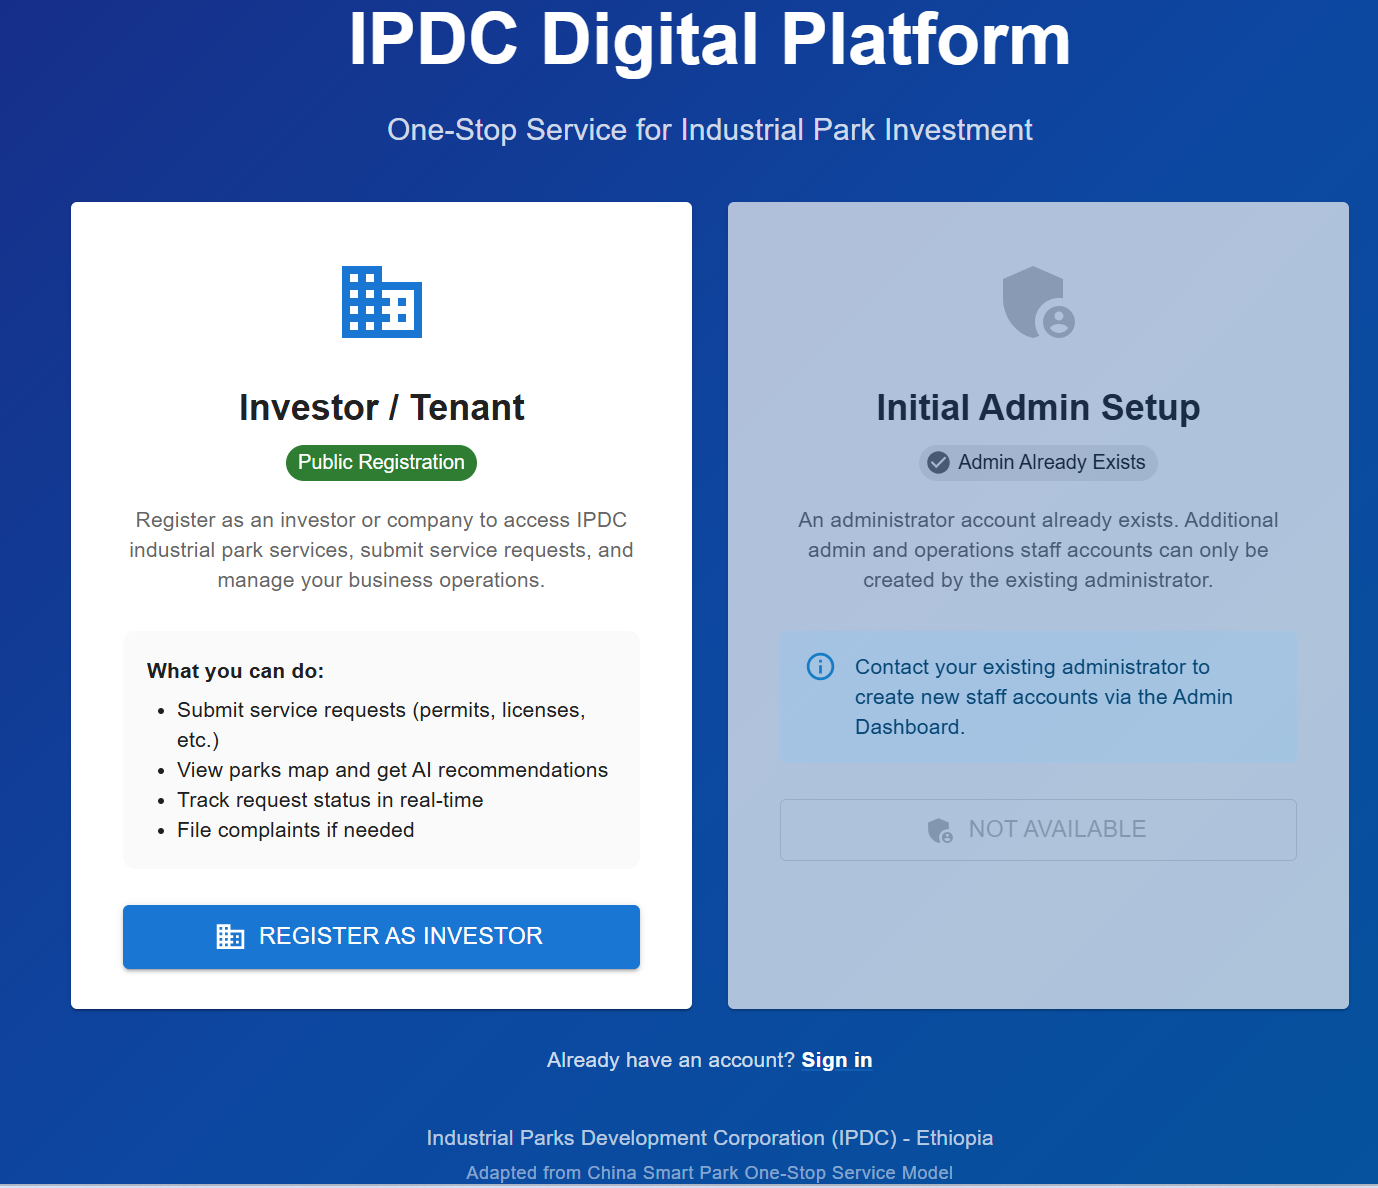
\includegraphics[width=\textwidth]{figures/fig_sign_up.png}
\end{minipage}
\caption[Authentication Interfaces]{Authentication Interfaces --- Sign-In (left) and Tenant Registration (right)}
\label{fig:auth-interfaces}
\end{figure}

\subsection{Service Request Management}

Service request management forms the backbone of the platform. The \texttt{CreateRequestForm} component (\texttt{src/components/tenant/}) uses React Hook Form for state management and Zod for schema validation. Requests can be categorized across multiple service types (maintenance, IT support, security, cleaning, waste management, and others), assigned one of four priority levels, given free-text descriptions, and accompanied by file attachments uploaded through the \texttt{FileUpload} component to Firebase Storage.

Each request follows a defined status progression: \texttt{pending} $\rightarrow$ \texttt{approved} $\rightarrow$ \texttt{in-progress} $\rightarrow$ \texttt{completed}. Administrators may also \texttt{reject} a request with a stated reason. Every status transition triggers a notification and updates the record in Firestore --- or in the local queue when offline. Figure~\ref{fig:tenant-workflow} shows the tenant dashboard alongside the service request creation form.

\begin{figure}[H]
\centering
\begin{minipage}[t]{0.48\textwidth}
\centering
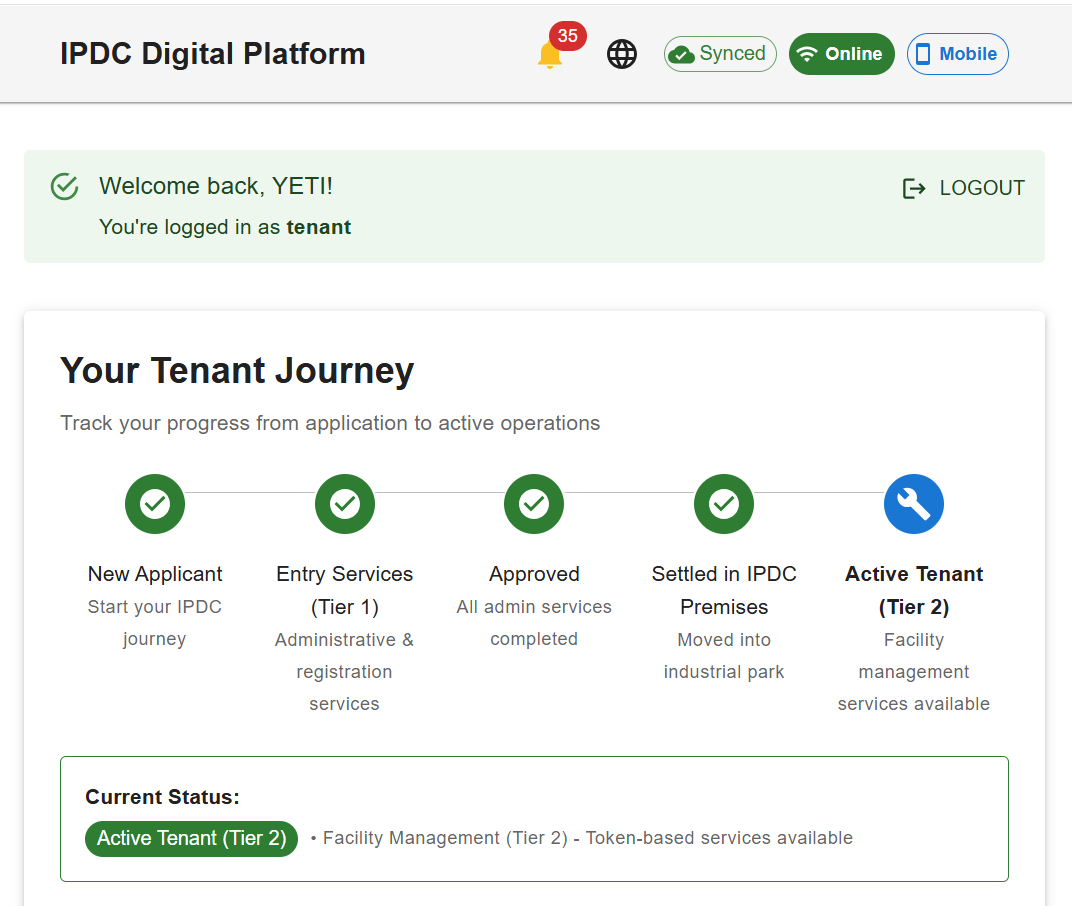
\includegraphics[width=\textwidth]{figures/fig_tenant_dashboard.png}
\end{minipage}
\hfill
\begin{minipage}[t]{0.48\textwidth}
\centering
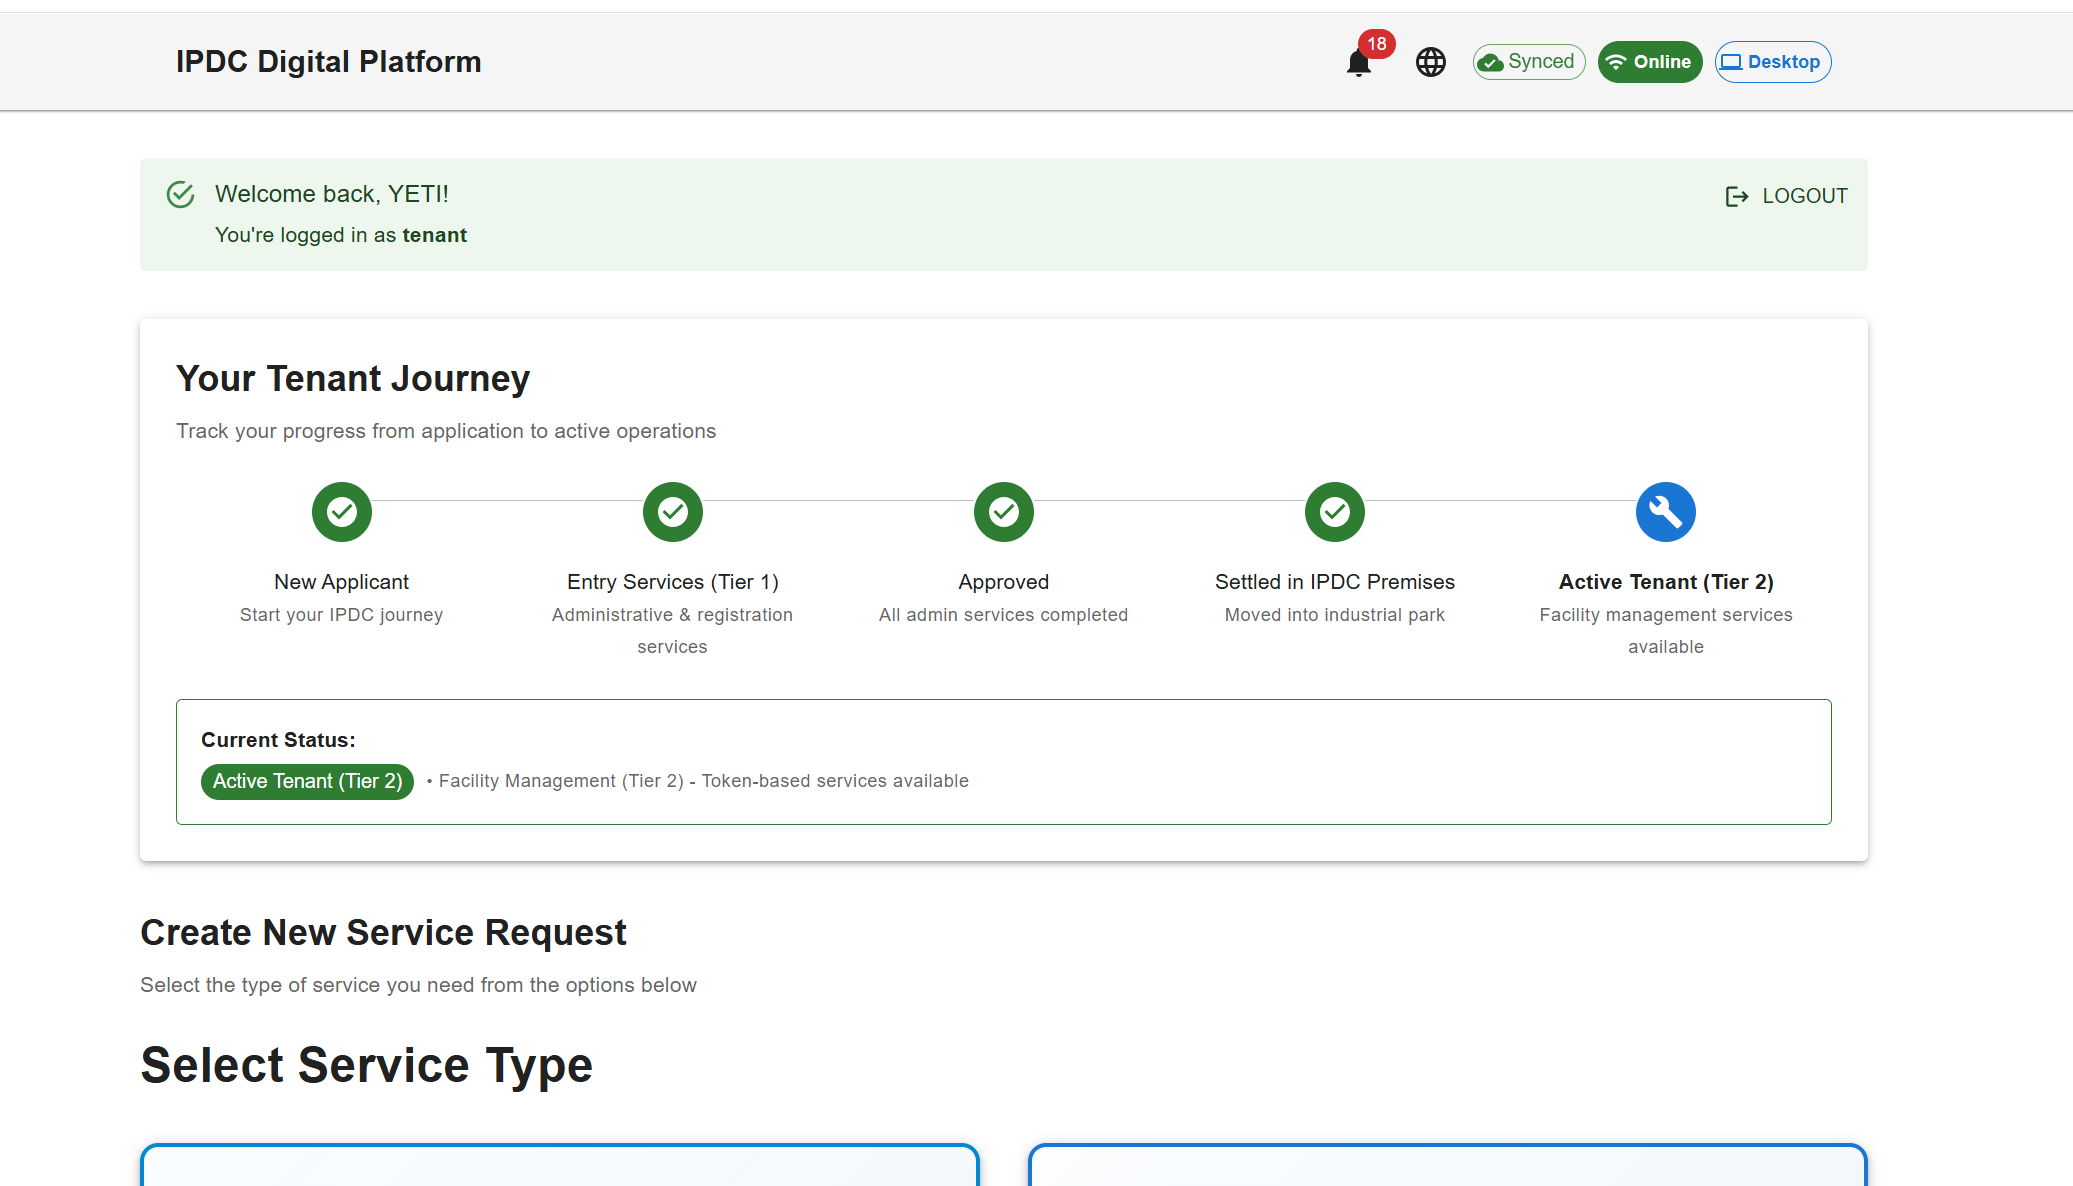
\includegraphics[width=\textwidth]{figures/fig_create_request.png}
\end{minipage}
\caption[Tenant Service Request Workflow]{Tenant Service Request Workflow --- Dashboard Overview (left) and Request Creation Form (right)}
\label{fig:tenant-workflow}
\end{figure}

\subsection{Digital Service Token System}

The token system provides an internal mechanism for tracking service fees without requiring an external payment gateway. Its implementation spans the \texttt{TokenDashboard} component and the \texttt{billingService} module.

\textbf{Token Tiers} reward engagement: basic through platinum (four tiers), each unlocking progressively larger discounts (0--20\%), higher monthly request limits, and priority support.

\textbf{Service Costs} vary by both service type and priority level. Table~\ref{tab:token-costs} shows the pricing matrix.

\begin{table}[H]
\centering
\caption{Service Token Pricing Matrix (tokens per request)}
\label{tab:token-costs}
\small
\begin{tabular}{lcccc}
\toprule
\textbf{Service Type} & \textbf{Low} & \textbf{Medium} & \textbf{High} & \textbf{Urgent} \\
\midrule
Maintenance & 50 & 80 & 120 & 150 \\
IT Support & 60 & 100 & 140 & 180 \\
Security & 40 & 65 & 95 & 120 \\
Cleaning & 25 & 45 & 65 & 80 \\
Waste Management & 35 & 60 & 85 & 110 \\
\bottomrule
\end{tabular}
\end{table}

A complete audit trail covers all transaction types (allocation, deduction, refund, bonus, penalty, purchase). Administrators credit tokens after confirming external payment receipt. Figure~\ref{fig:token-dashboard} shows the token dashboard interface.

\begin{figure}[H]
\centering

\includegraphics[width=0.75\textwidth]{figures/fig_token_dashboard.png}
\caption{Digital Service Token Dashboard}
\label{fig:token-dashboard}
\end{figure}

\subsection{AI Model Integration}

Three machine learning models are connected to the platform through a FastAPI backend. The frontend AI service module (\texttt{src/services/aiService.ts}) exposes typed interfaces for each model endpoint, with error handling and timeout management built in.

\textbf{Model 1 --- Service Classifier:} Trained on labeled service request data, this model sorts incoming requests into eleven service categories and assigns priority levels. Because the endpoint returns a confidence score, the interface presents predictions as suggestions that users can accept or override.

\textbf{Model 2 --- Predictive Maintenance:} This was the model stakeholders responded to most immediately during the usability evaluation --- the idea of warning operations staff before equipment fails, rather than after, resonated without any prompting. Given asset attributes, it produces a failure probability, risk level (low/medium/high), estimated days until failure, and a recommended maintenance action.

\textbf{Model 3 --- Park Recommendation:} Built to help prospective tenants choose a suitable industrial park, this model evaluates a tenant profile against park characteristics using a weighted scoring algorithm. Five dimensions --- industry alignment (30\%), capacity and availability (25\%), infrastructure match (20\%), cost efficiency (15\%), and location preference (10\%) --- produce ranked recommendations with detailed justifications.

All three models degrade gracefully: if the API is unreachable, the interface disables AI features without disrupting core service request and management workflows. Figure~\ref{fig:ai-interfaces} shows the service classifier and park recommendation interfaces; Figure~\ref{fig:predictive-views} presents the predictive maintenance module.

\begin{figure}[H]
\centering
\begin{minipage}[t]{0.48\textwidth}
\centering
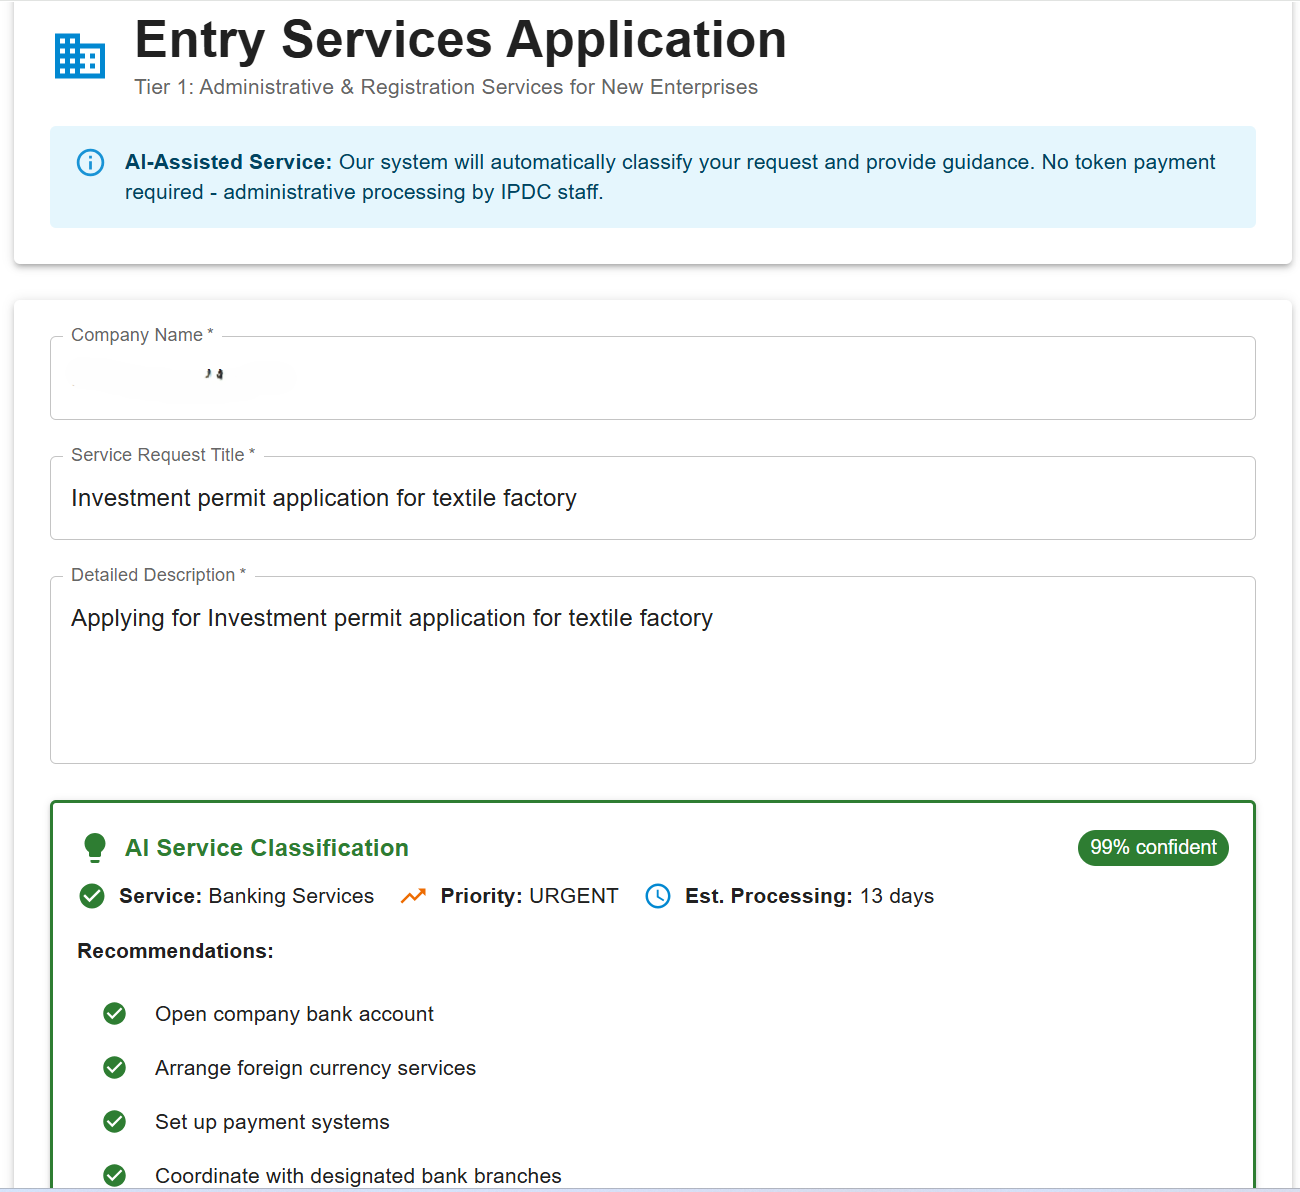
\includegraphics[width=\textwidth]{figures/fig_service_classifier.png}
\end{minipage}
\hfill
\begin{minipage}[t]{0.48\textwidth}
\centering
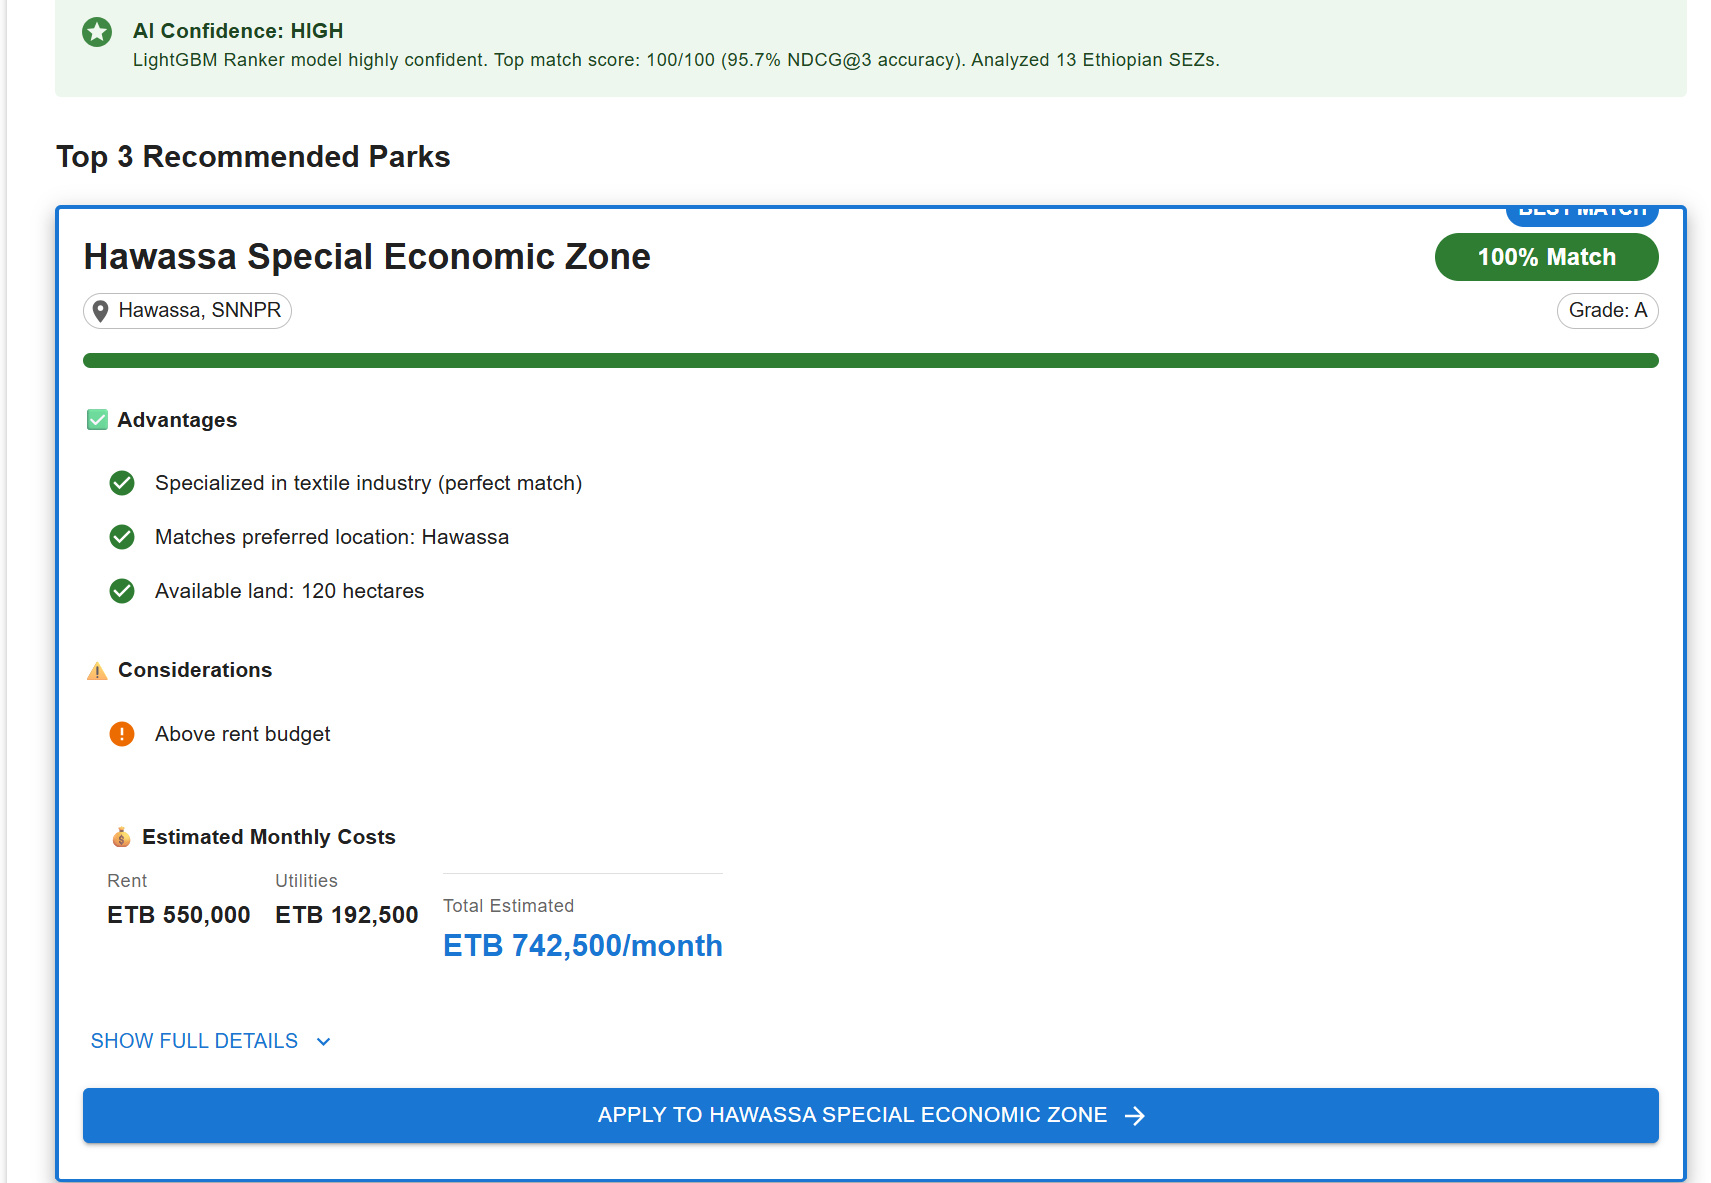
\includegraphics[width=\textwidth]{figures/fig_park_recommendation.png}
\end{minipage}
\caption[AI Model Interfaces]{AI Model Interfaces --- Service Classifier (left) and Park Recommendation (right)}
\label{fig:ai-interfaces}
\end{figure}

\begin{figure}[H]
\centering
\begin{minipage}[t]{0.48\textwidth}
\centering
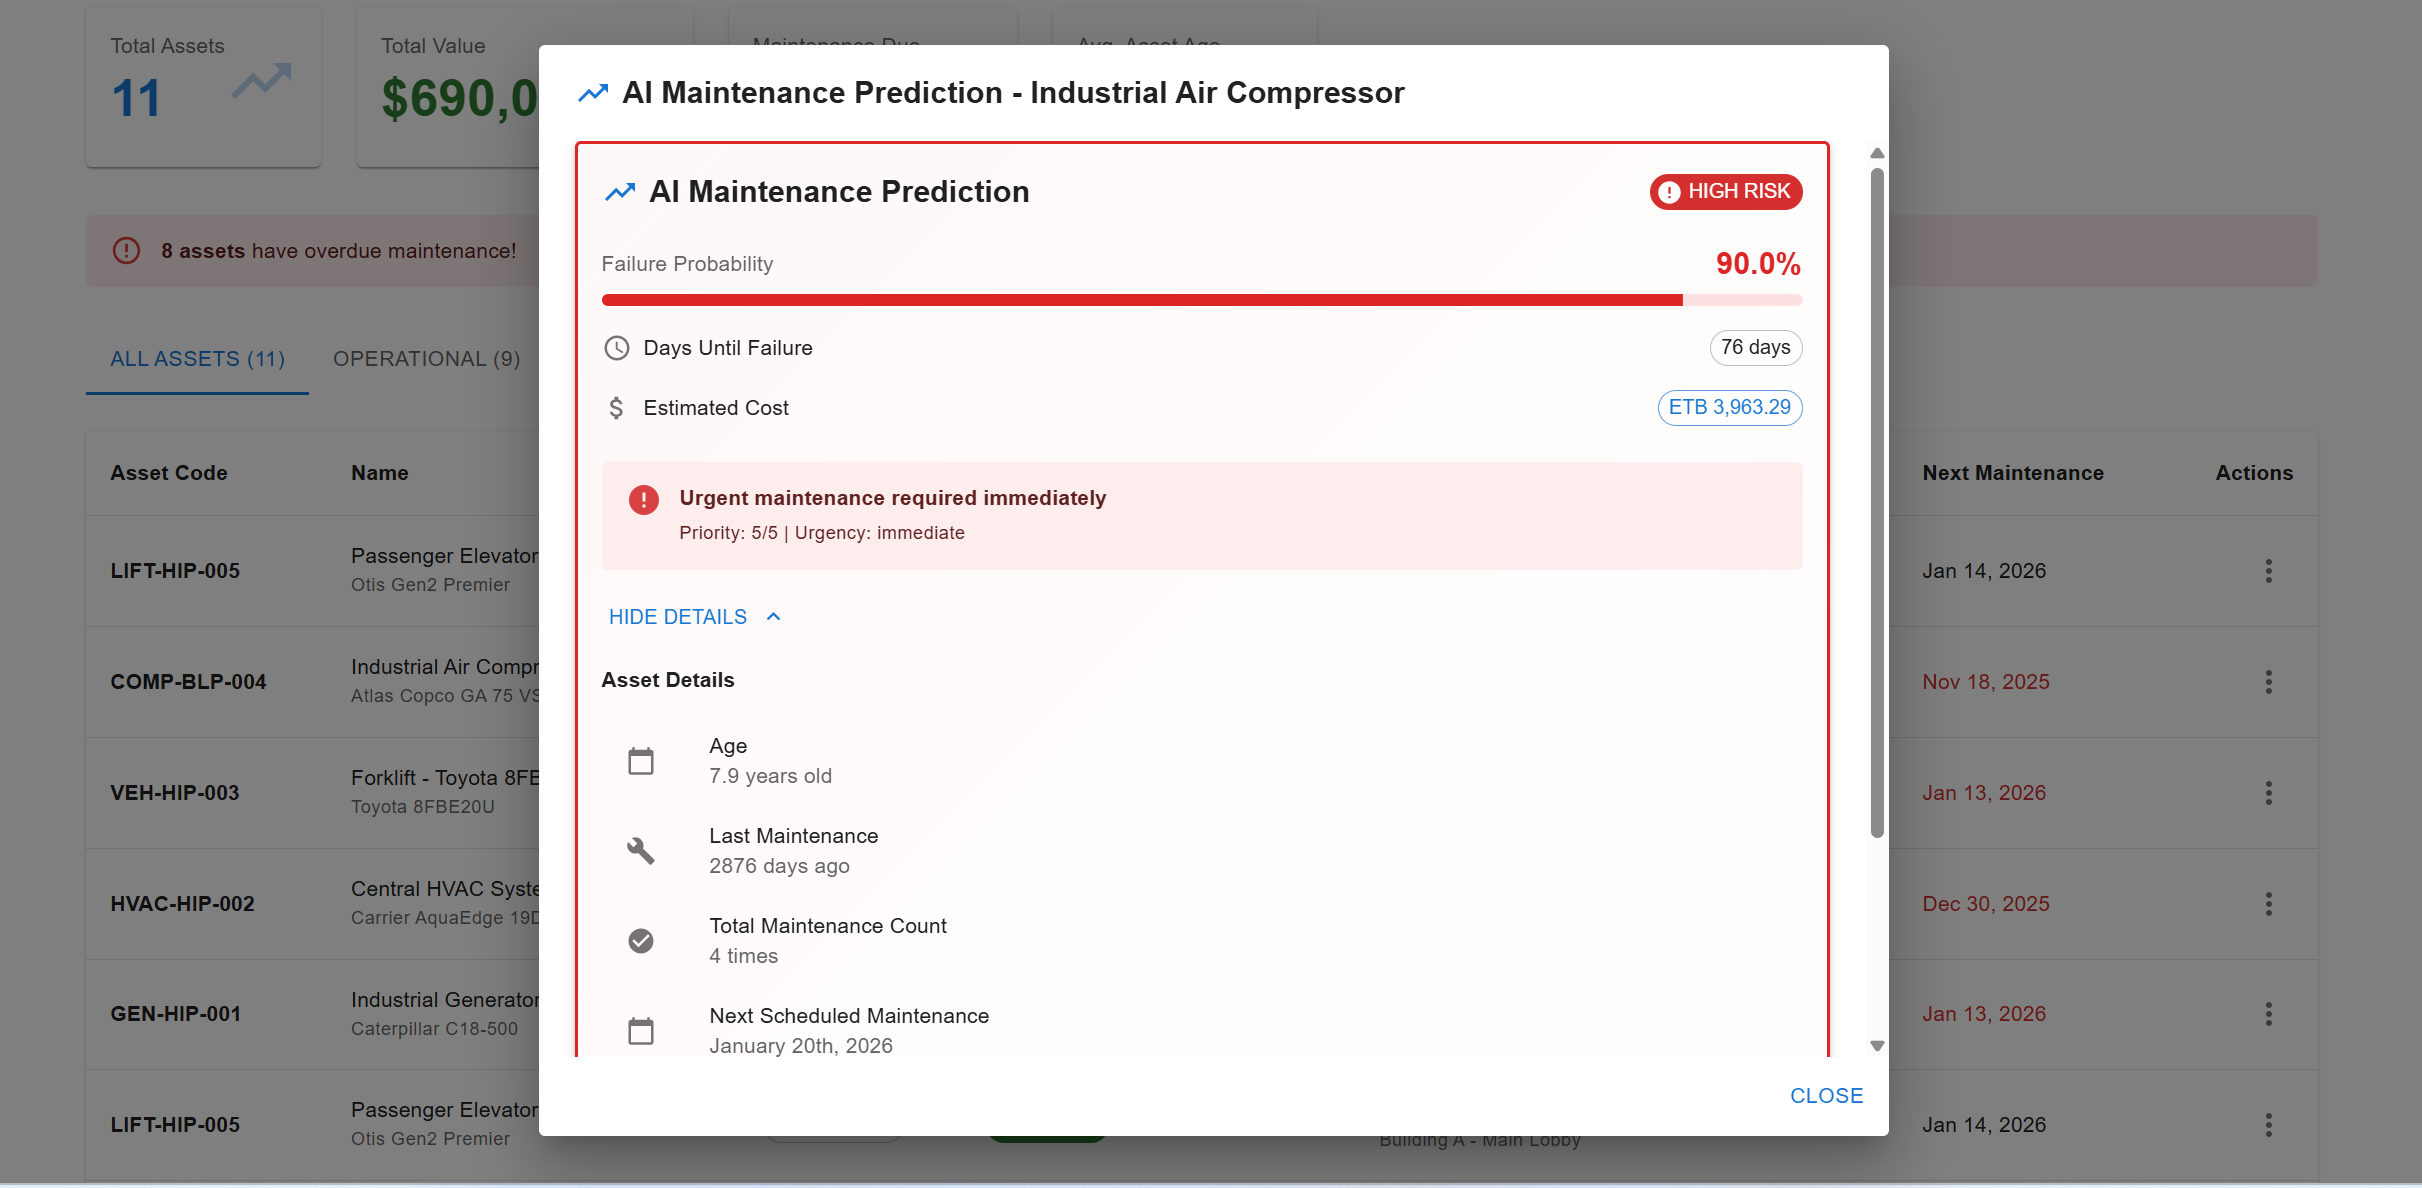
\includegraphics[width=\textwidth]{figures/fig_predictive_maintenance.png}
\end{minipage}
\hfill
\begin{minipage}[t]{0.48\textwidth}
\centering

\includegraphics[width=\textwidth]{figures/fig_predictive_maintenance_2.png}
\end{minipage}
\caption[Predictive Maintenance Views]{Predictive Maintenance Views --- Asset Overview (left) and Maintenance Detail (right)}
\label{fig:predictive-views}
\end{figure}

\subsection{Complaint Management System}

The complaint management module gives tenants a structured channel for raising issues with completed service requests. Nine complaint categories are available: service quality, incomplete work, delays, unprofessional conduct, billing dispute, facility issue, safety concern, communication gap, and other. Each complaint supports evidence uploads (images, documents, videos) and follows a resolution workflow: \texttt{pending} $\rightarrow$ \texttt{under-review} $\rightarrow$ \texttt{resolved} or \texttt{rejected}. Resolution actions range from full or partial token refund to service rework and compensation, with a 48-hour SLA target tracked for each complaint. Figure~\ref{fig:communication-interfaces} shows the complaint management and announcement interfaces.

\begin{figure}[H]
\centering
\begin{minipage}[t]{0.48\textwidth}
\centering
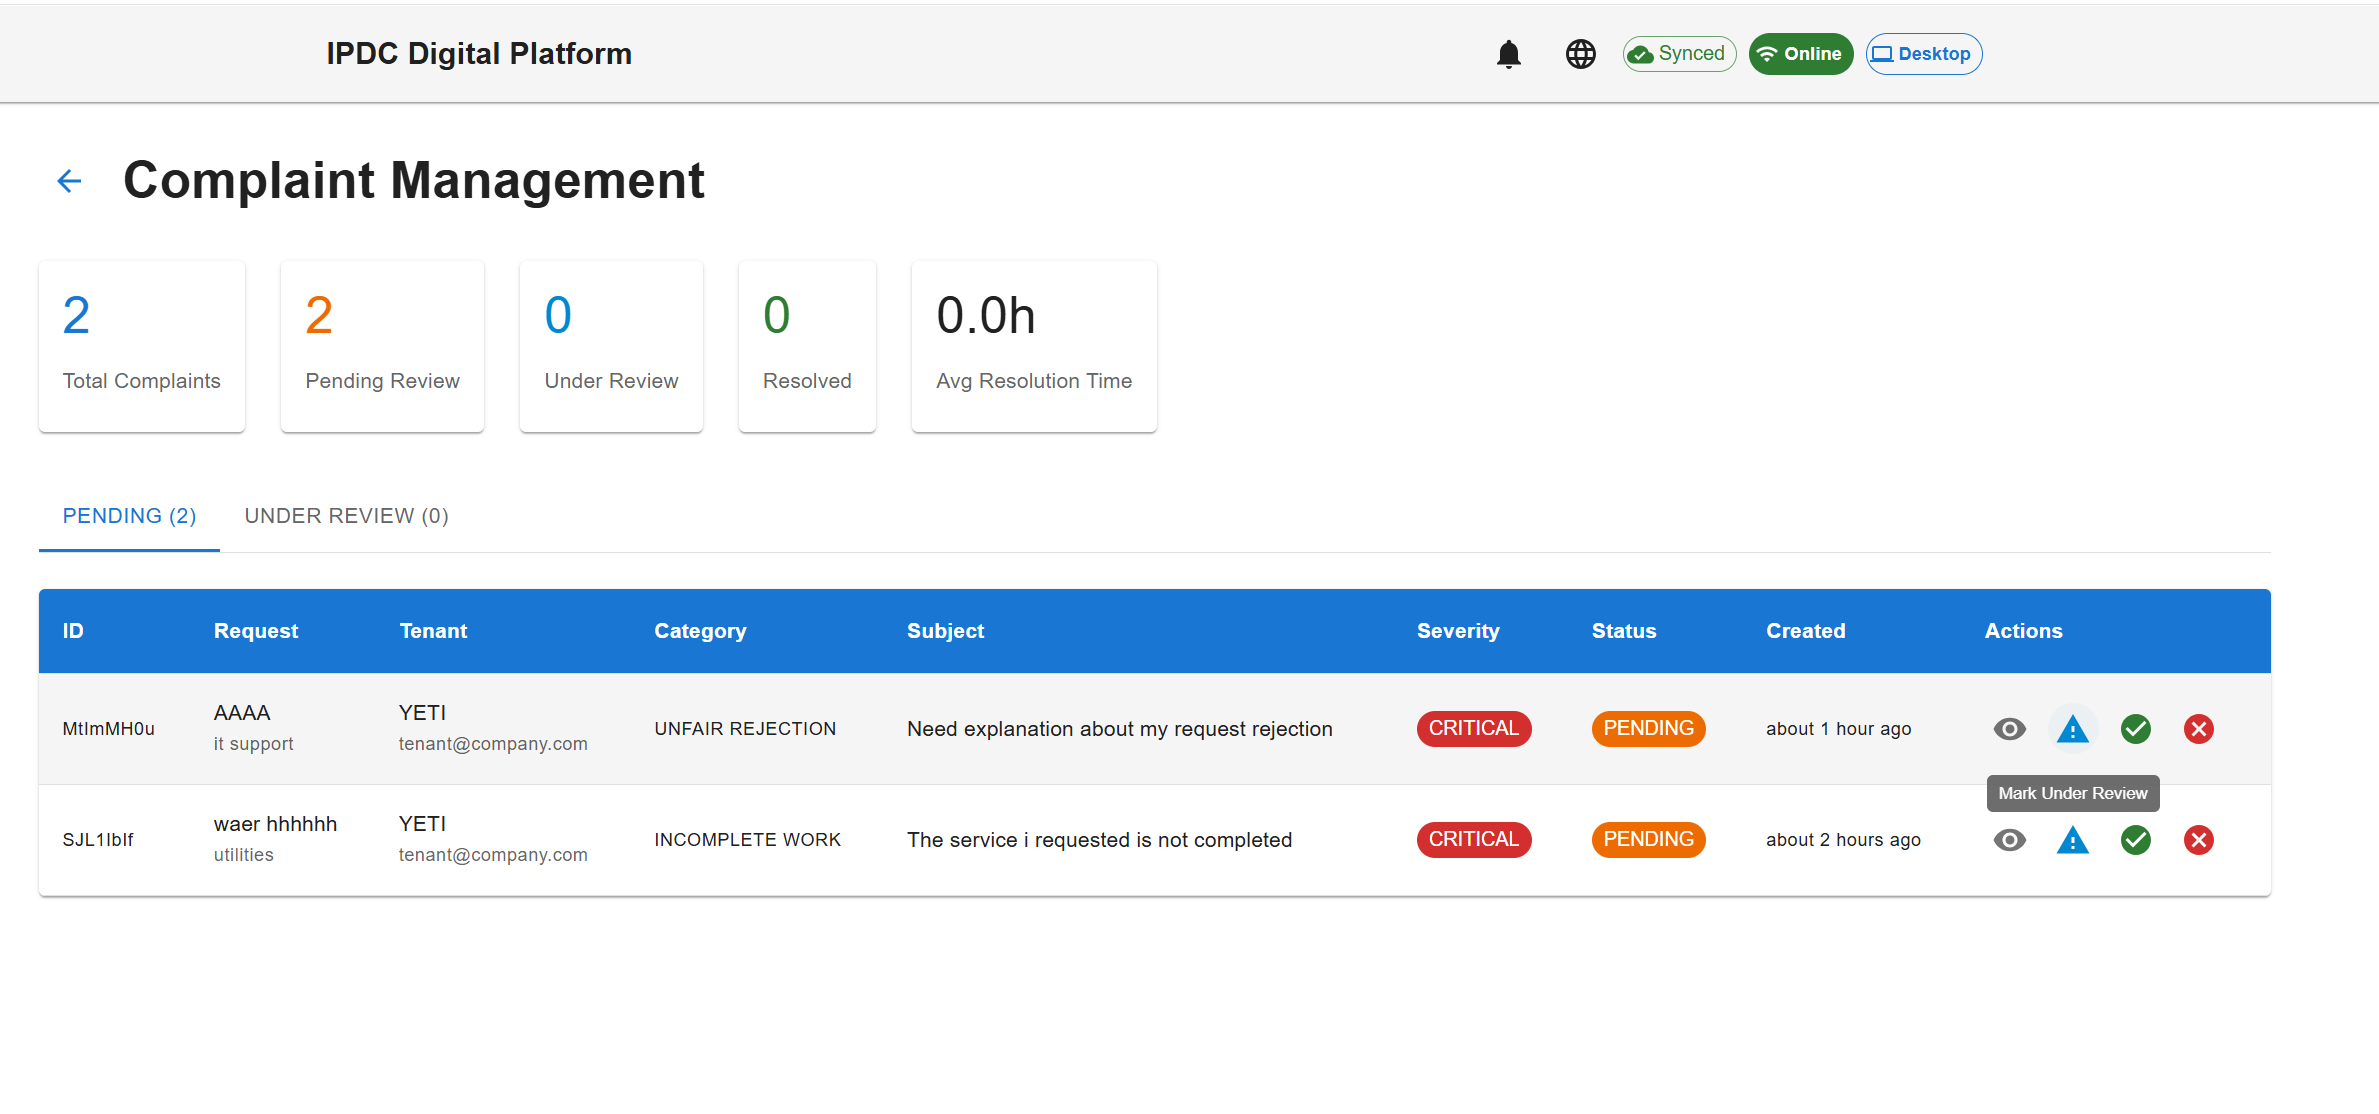
\includegraphics[width=\textwidth]{figures/fig_complaint_management.png}
\end{minipage}
\hfill
\begin{minipage}[t]{0.48\textwidth}
\centering

\includegraphics[width=\textwidth]{figures/fig_announcements.png}
\end{minipage}
\caption[Communication and Feedback Interfaces]{Communication and Feedback Interfaces --- Complaint Management (left) and Announcement System (right)}
\label{fig:communication-interfaces}
\end{figure}

\subsection{Announcement System}

The announcement module lets administrators create and distribute notices targeted at specific audience groups (all users, tenants only, operations only, or admin only). Each announcement carries a priority level, an optional expiration date, and an active/inactive toggle. The \texttt{AnnouncementBanner} component displays active announcements prominently across the interface, as shown in Figure~\ref{fig:communication-interfaces}.

\subsection{Interactive Park Map}

The park map module uses Leaflet and React-Leaflet to render an interactive geographic visualization of Ethiopian industrial parks. Clicking a marker opens a \texttt{ParkDetailsModal} displaying location details, available infrastructure, operational status, and tenant composition. Park coordinate data is stored in a static file within the application, so the map remains available during offline operation. Figure~\ref{fig:parks-map} shows the interface.

\begin{figure}[H]
\centering

\includegraphics[width=0.85\textwidth]{figures/fig_parks_map.png}
\caption{Interactive Industrial Parks Map}
\label{fig:parks-map}
\end{figure}

\subsection{Administrative Dashboard}

The admin dashboard (\texttt{src/pages/AdminDashboard.tsx}) is the central management interface. From here, administrators can view all service requests across the system, manage tenant accounts, create announcements, resolve complaints, oversee token and billing records, and manage park assets. Tabbed navigation organizes these functions; summary statistics and charts (powered by Recharts) provide at-a-glance operational visibility. Park operators have a dedicated dashboard for day-to-day service operations within their assigned park. Both are shown in Figure~\ref{fig:management-dashboards}.

\begin{figure}[H]
\centering
\begin{minipage}[t]{0.48\textwidth}
\centering
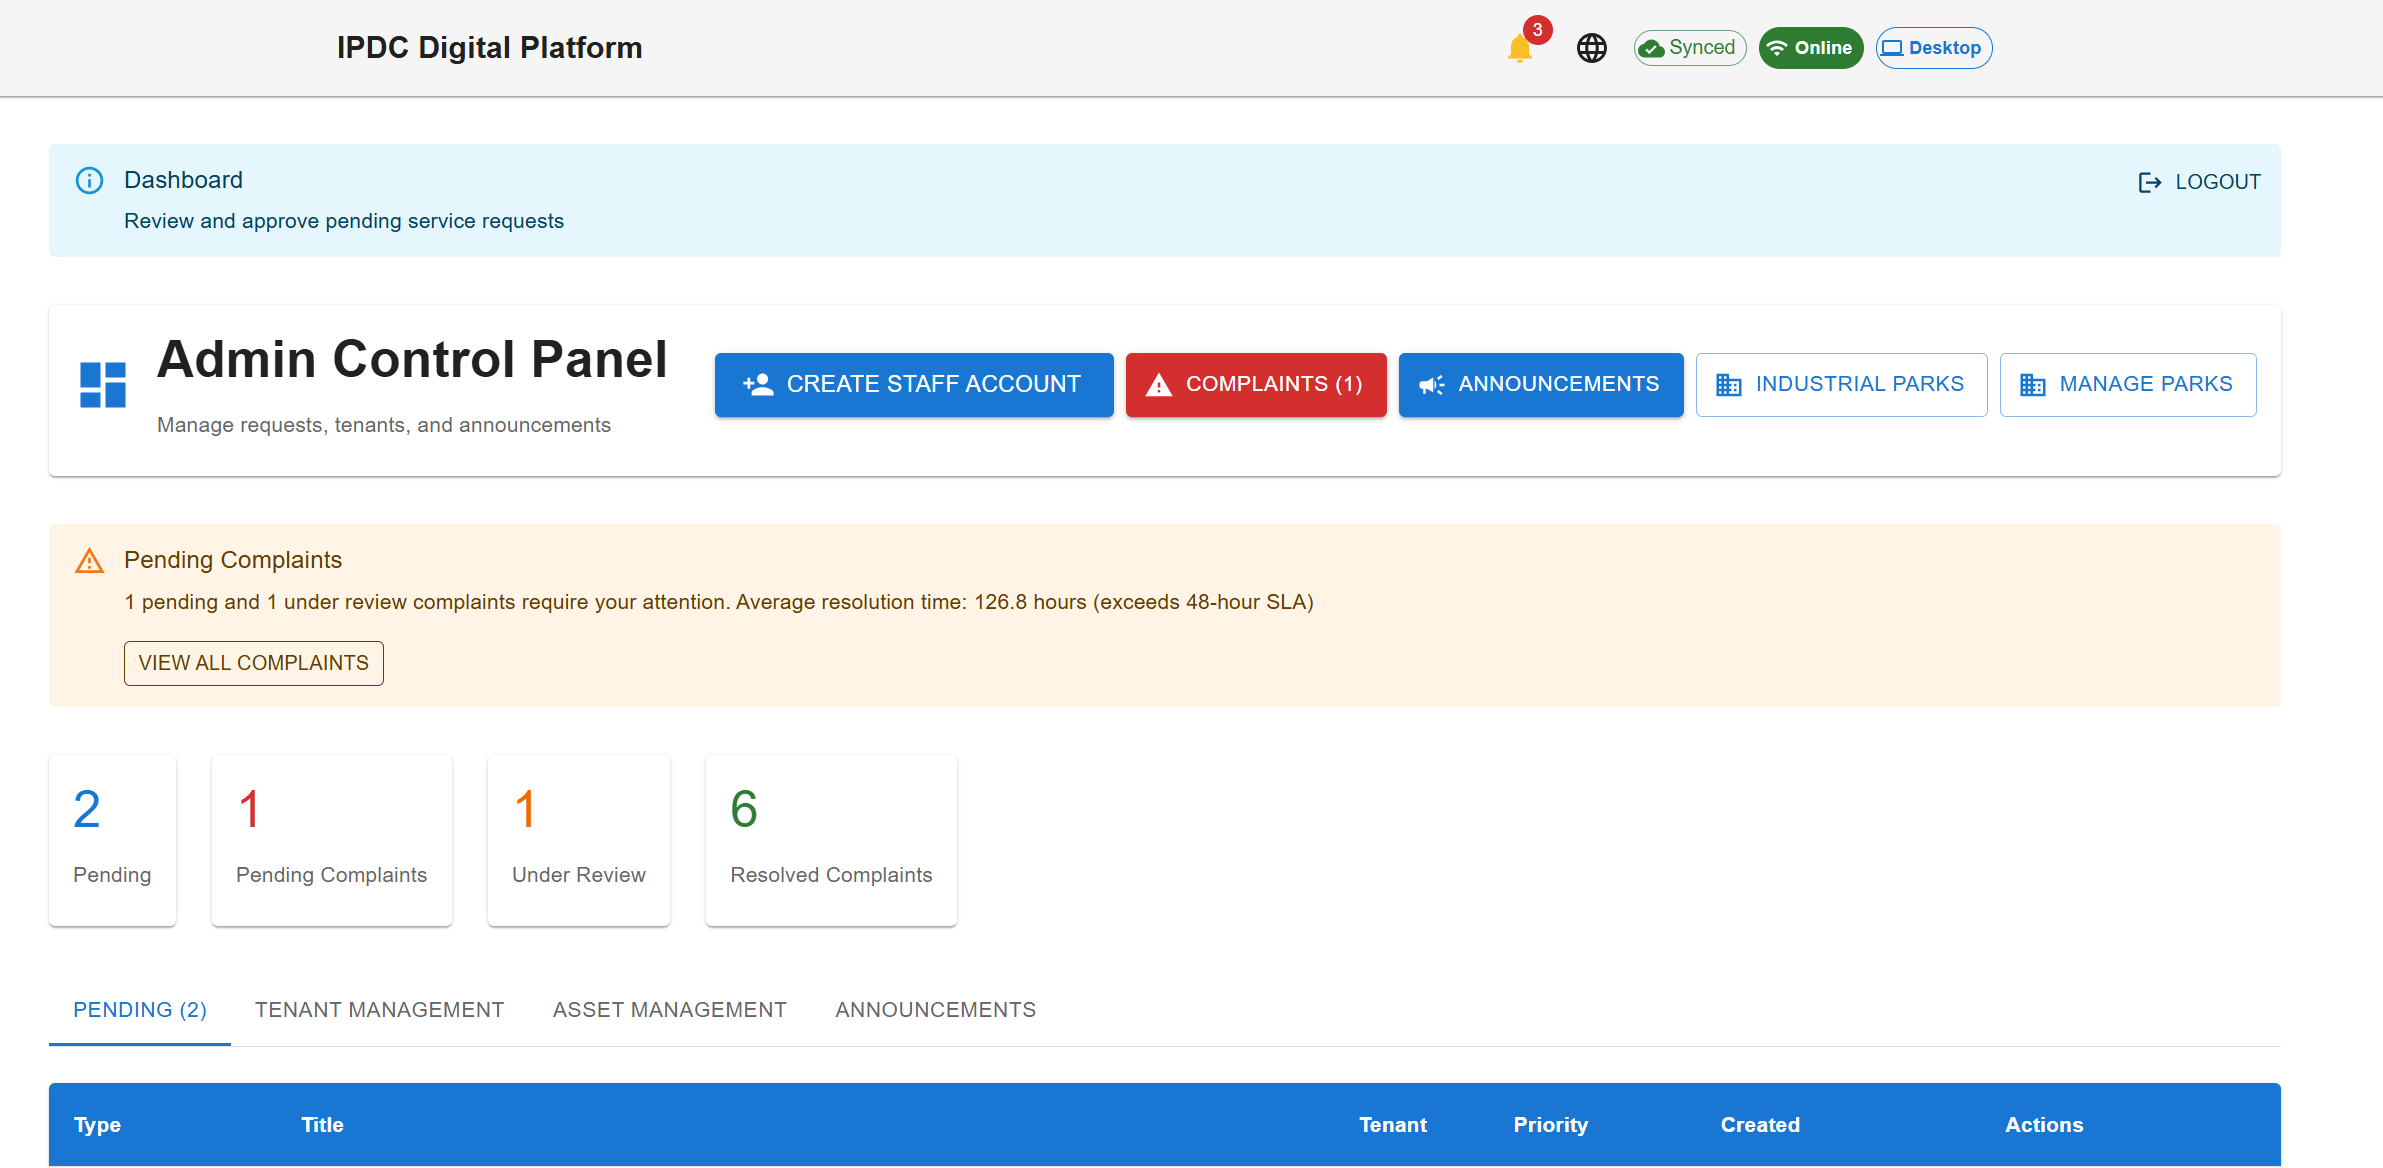
\includegraphics[width=\textwidth]{figures/fig_admin_dashboard.png}
\end{minipage}
\hfill
\begin{minipage}[t]{0.48\textwidth}
\centering
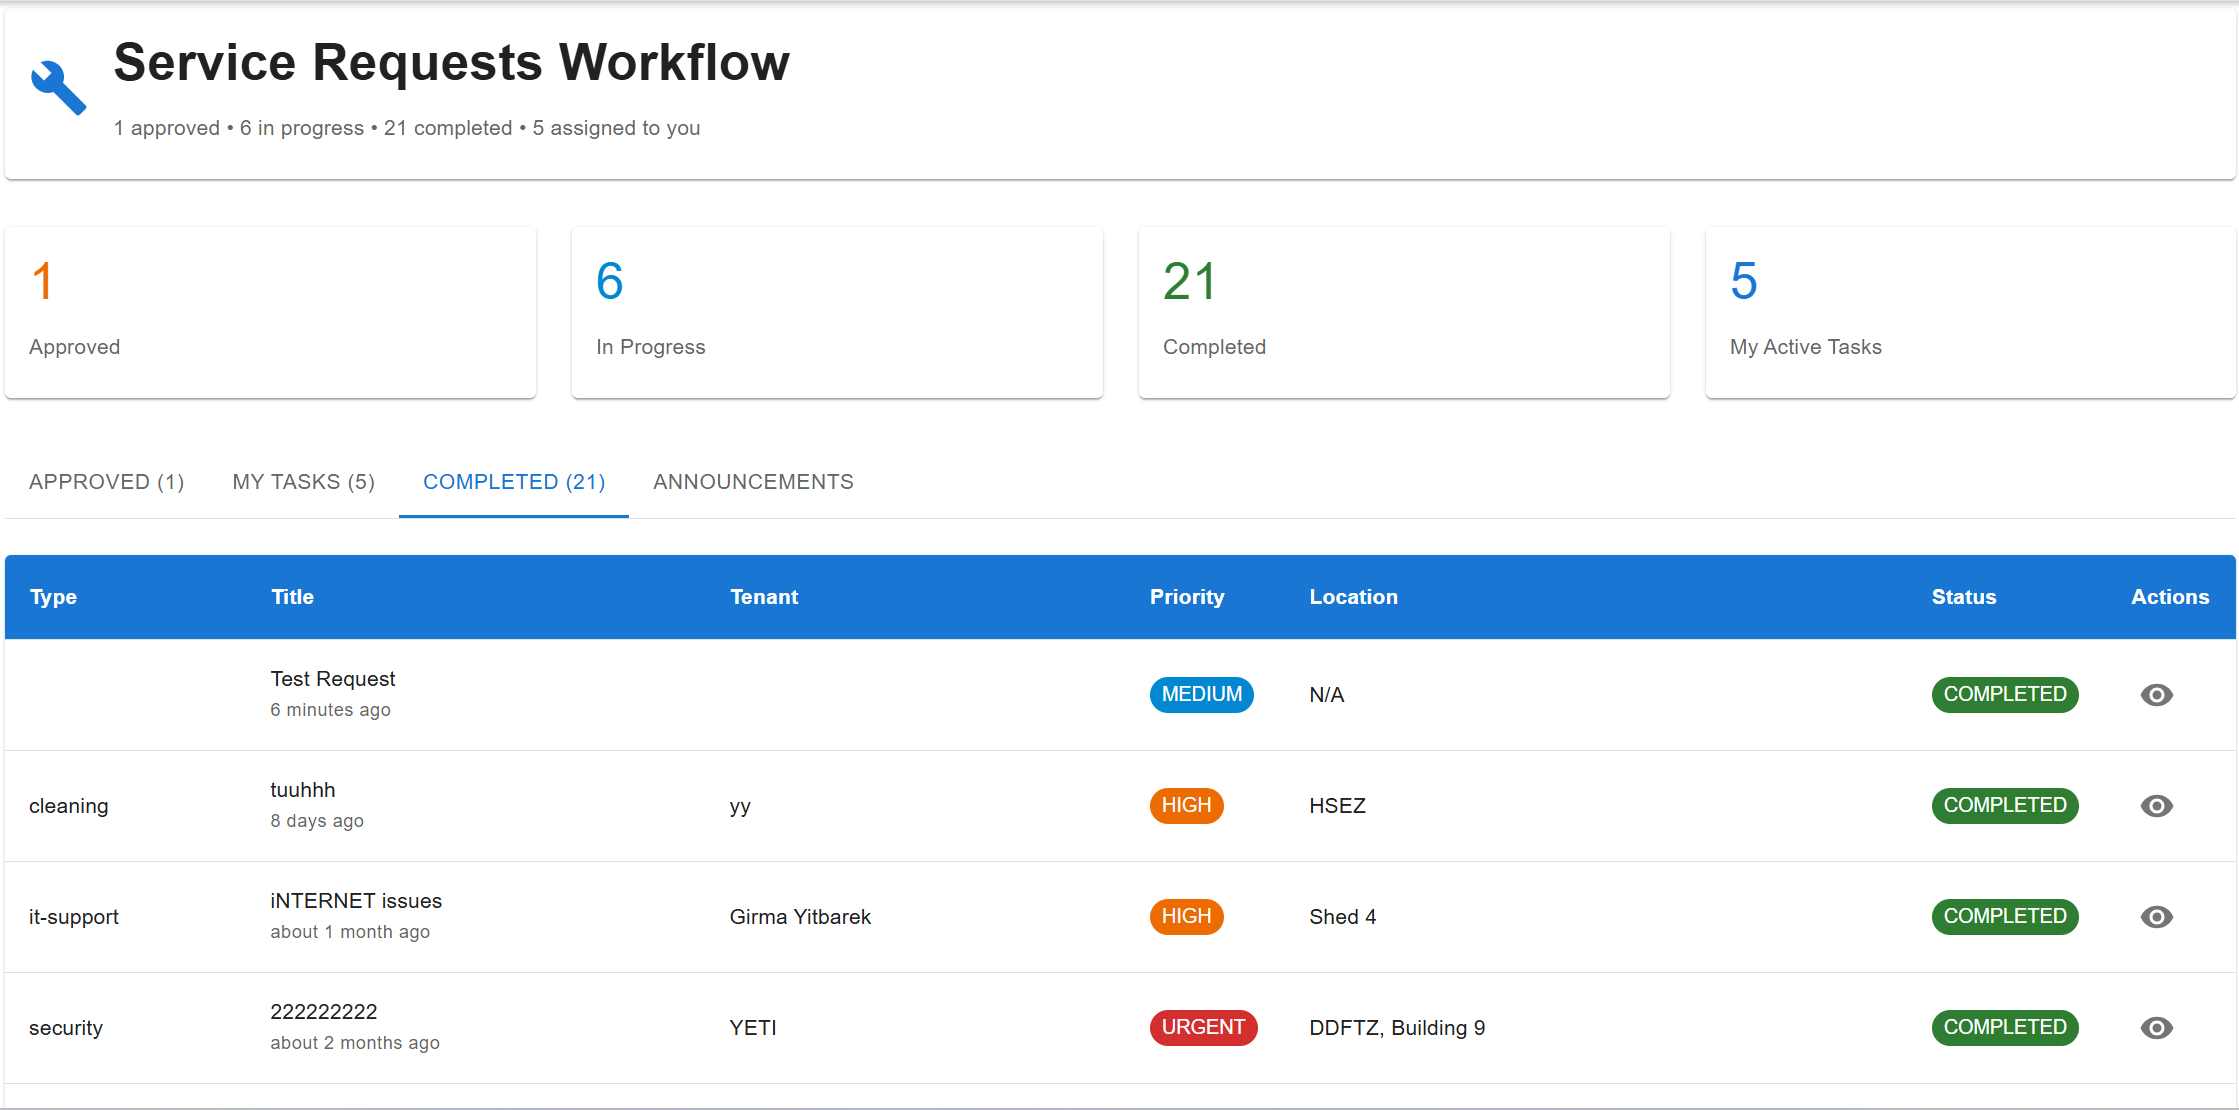
\includegraphics[width=\textwidth]{figures/fig_operators_dashboard.png}
\end{minipage}
\caption[Management Dashboard Interfaces]{Management Dashboard Interfaces --- Administrator (left) and Park Operators (right)}
\label{fig:management-dashboards}
\end{figure}

\section{AI Model Training and Evaluation}
\label{sec:ai-training}

This section documents how the three machine learning models were trained, what their data looks like, how they are structured, and how well they perform. All models were trained on synthetic datasets designed to reflect realistic IPDC operational patterns, with architectures informed by leading Chinese smart city systems --- Alibaba ET Industrial Brain, Tencent WeCity, and Huawei FusionPlant.

\subsection{Training Data}

Three domain-specific datasets were produced using the data synthesis pipeline (\texttt{ai-models/data/generate\_synthetic\_data.py}). Table~\ref{tab:training-data} summarizes their characteristics.

\begin{table}[H]
\centering
\caption{Training Dataset Characteristics}
\label{tab:training-data}
\small
\begin{tabular}{p{3.5cm}p{2cm}p{2cm}p{5cm}}
\toprule
\textbf{Dataset} & \textbf{Records} & \textbf{Features} & \textbf{Target Variables} \\
\midrule
Service Requests & 2,200 & 10 & Service type (11 classes), priority (4 classes), processing days (continuous) \\
Asset Maintenance & 500 & 14 & Failure flag (binary), days to failure (continuous), risk level (3 classes) \\
Park Placements & 10,400\textsuperscript{a} & 11 & Match score (relevance grade 0--4) \\
\bottomrule
\end{tabular}

\vspace{0.3cm}
\footnotesize
\textsuperscript{a} 800 tenant profiles $\times$ 13 industrial parks = 10,400 ranking pairs.
\end{table}

The service requests dataset includes text fields (title, description) processed through TF-IDF vectorization, alongside temporal metadata (hour of day, day of week) and text statistics (word count, character length). The asset maintenance dataset captures equipment attributes such as age, condition scores, maintenance history, and sensor readings (temperature, vibration level). The park placements dataset pairs every tenant profile with all 13 Ethiopian industrial parks in a learning-to-rank format, where the chosen park receives the highest relevance grade.

\subsection{Model 1: Smart Service Classifier}

\subsubsection{Architecture}

The service classifier is an XGBoost ensemble comprising three specialized sub-models. Text features are extracted using TF-IDF vectorization with a 1,500-term vocabulary (unigrams and bigrams, minimum document frequency of 2, maximum document frequency of 0.90). Four metadata features --- hour of day, day of week, text length, and word count --- are scaled with StandardScaler and concatenated with the TF-IDF vectors, yielding 1,504 input features per request.

\begin{table}[H]
\centering
\caption{Service Classifier Configuration and Results}
\label{tab:model1-config}
\label{tab:model1-results}
\small

\textbf{(a) Sub-Model Configurations}\\[0.3em]
\begin{tabular}{p{3.5cm}p{2.5cm}p{2cm}p{2cm}p{2cm}}
\toprule
\textbf{Sub-Model} & \textbf{Objective} & \textbf{Depth} & \textbf{LR} & \textbf{Trees} \\
\midrule
Category Classifier & Multi-class softmax & 6 & 0.1 & 100 \\
Priority Predictor & Multi-class softmax & 5 & 0.1 & 80 \\
Time Estimator & Squared error & 4 & 0.1 & 60 \\
\bottomrule
\end{tabular}

\vspace{0.5cm}
\textbf{(b) Evaluation Results}\\[0.3em]
\begin{tabular}{p{5cm}cc}
\toprule
\textbf{Metric} & \textbf{Value} & \textbf{Benchmark\textsuperscript{a}} \\
\midrule
Service Type Accuracy & 100\% & 85--92\% \\
Priority Classification Accuracy & 40\% & --- \\
Processing Time MAE & 2.63 days & $\pm$3 days \\
Processing Time $R^{2}$ & 0.577 & --- \\
Average Confidence Score & 0.95 & --- \\
\bottomrule
\end{tabular}

\vspace{0.3cm}
\footnotesize
\textsuperscript{a} Alibaba ET Industrial Brain benchmark on similar classification tasks.
\end{table}

The training data was split into 70\% training (1,386 samples), 15\% validation (297 samples), and 15\% test (297 samples).

Category classification reaches 100\% on the synthetic set --- the eleven IPDC service types have distinct vocabulary patterns, making separation straightforward. The priority predictor's 40\% accuracy reflects the subjectivity of human judgment, not a shortcoming of the model. The time estimator's 2.63-day MAE offers tenants useful planning estimates. Figure~\ref{fig:model1-eval} presents the confusion matrix for service type classification and the scatter plot of predicted versus actual processing days.

\begin{figure}[H]
\centering
\begin{minipage}[t]{0.48\textwidth}
\centering
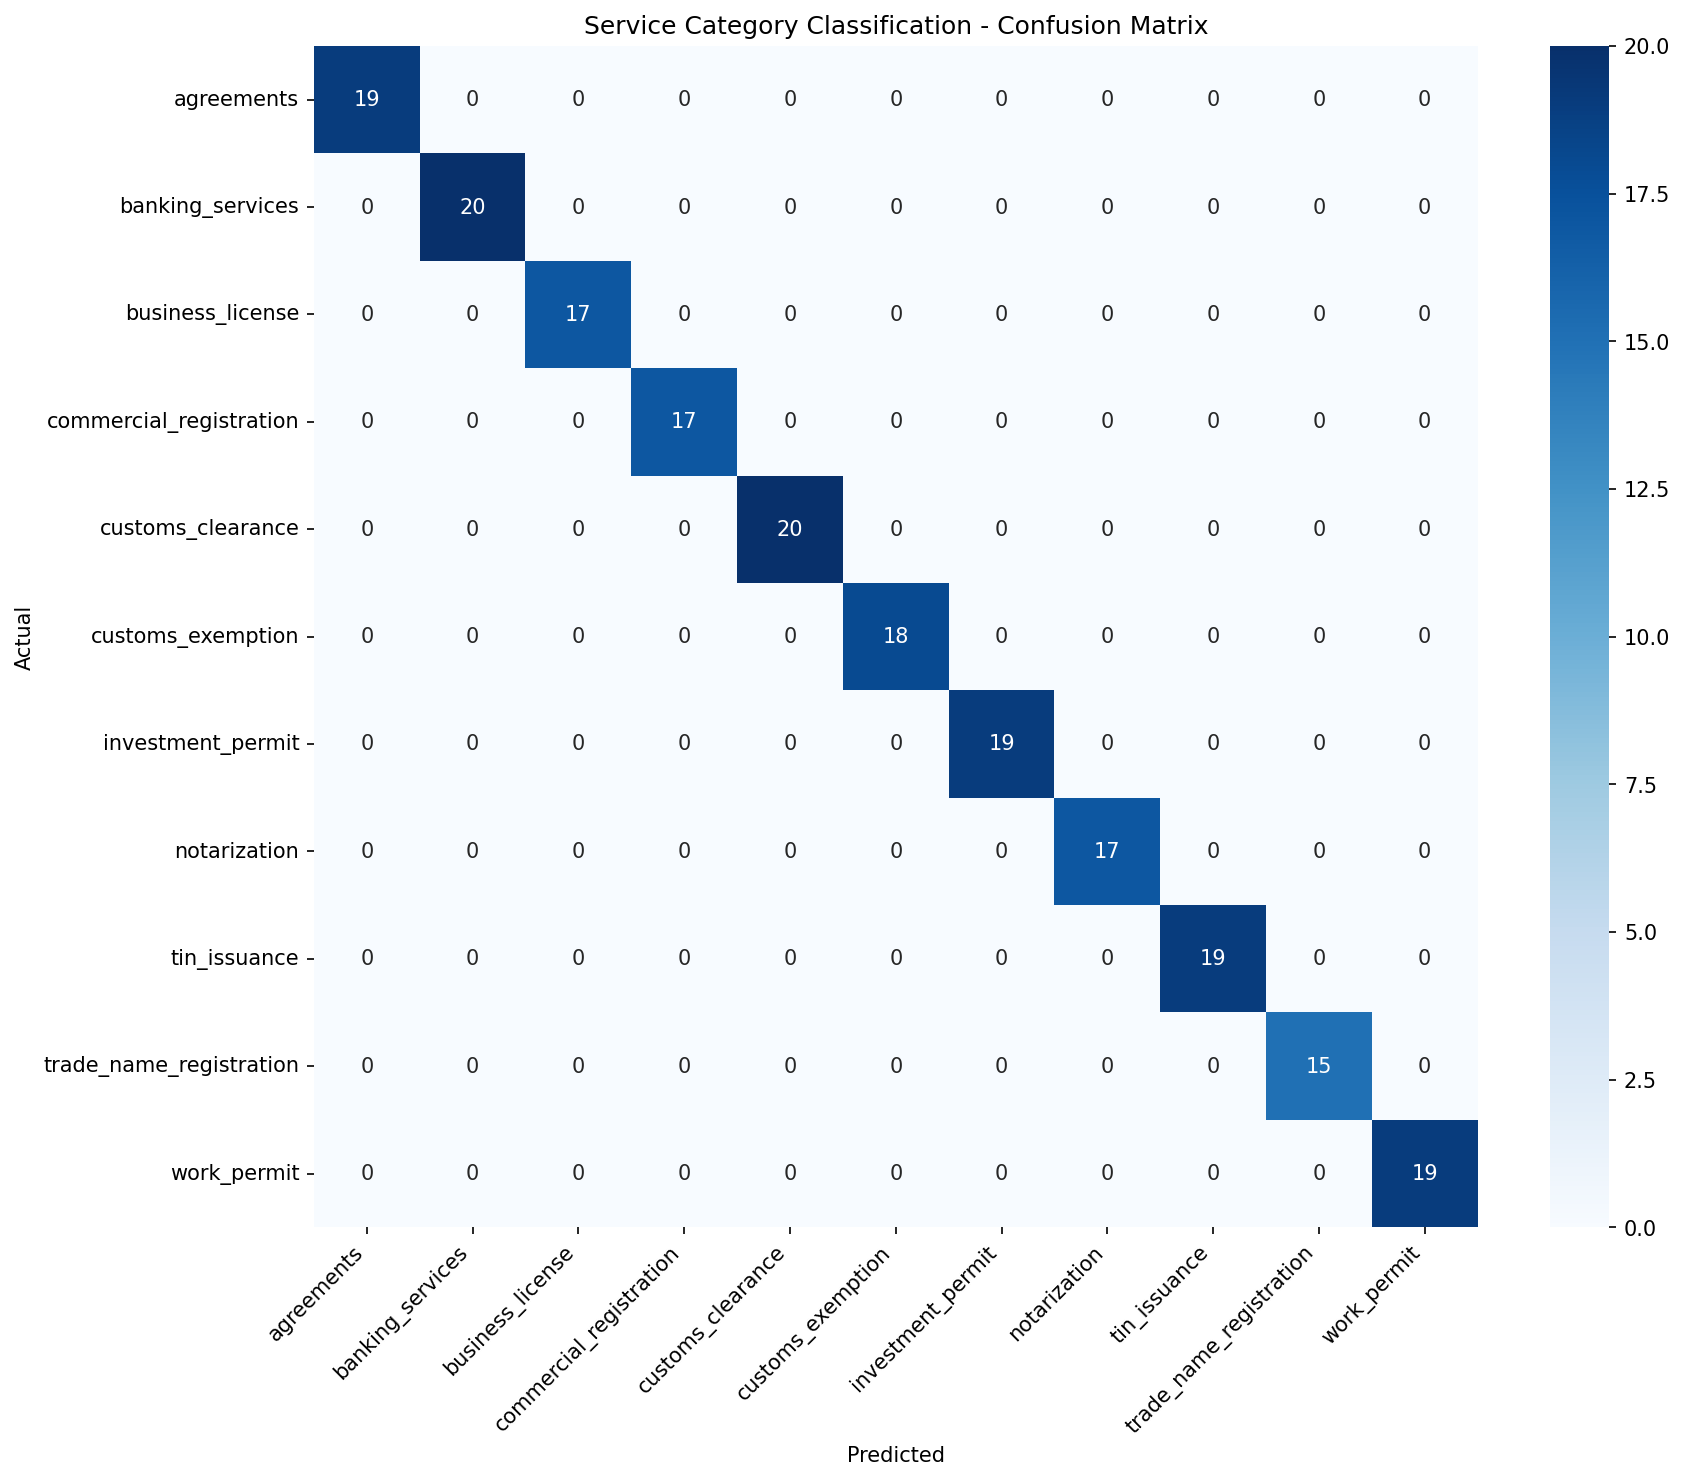
\includegraphics[width=\textwidth]{figures/model1_confusion_matrix_category.png}
\end{minipage}
\hfill
\begin{minipage}[t]{0.48\textwidth}
\centering
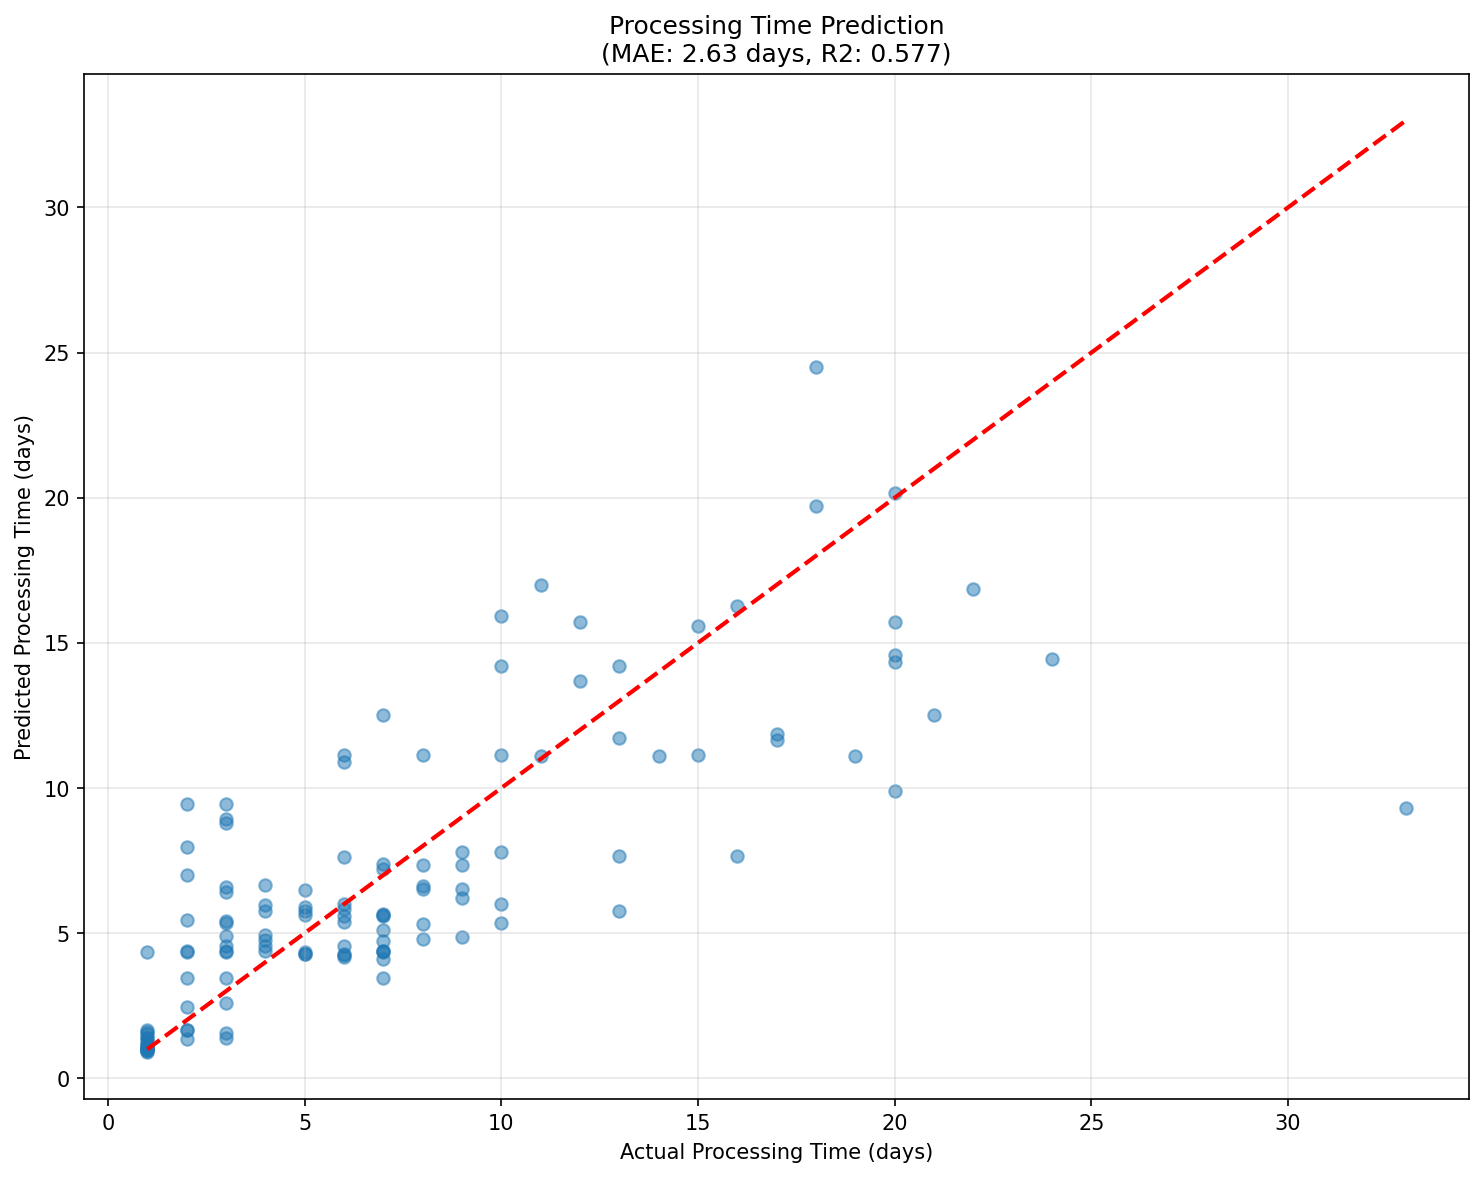
\includegraphics[width=\textwidth]{figures/model1_time_prediction_scatter.png}
\end{minipage}
\caption[Service Classifier Evaluation (Model 1)]{Service Classifier Evaluation (Model 1) --- Confusion Matrix (left) and Processing Time Prediction (right)}
\label{fig:model1-eval}
\end{figure}

\subsection{Model 2: Predictive Maintenance System}

\subsubsection{Architecture}

The predictive maintenance system combines two algorithms in a dual-algorithm ensemble: Random Forest for classification and Gradient Boosting for regression. Fourteen engineered features are derived from raw asset attributes, including age in days, days since last maintenance, cumulative maintenance count, operating hours, historical failure count, sensor readings (temperature, vibration level), and a composite condition score:

\begin{equation}
\text{Condition Score} = \frac{\text{age\_months}}{120} \times 30 + \frac{\text{days\_since\_maint}}{365} \times 30 + \text{failures} \times 10 + \frac{\text{hours}}{20000} \times 10
\label{eq:condition-score}
\end{equation}

Categorical features (asset category, status, condition level) are encoded with LabelEncoder; all features are normalized using StandardScaler.

\begin{table}[H]
\centering
\caption{Predictive Maintenance Configuration and Results}
\label{tab:model2-config}
\label{tab:model2-results}
\small

\textbf{(a) Sub-Model Configurations}\\[0.3em]
\begin{tabular}{p{3.5cm}p{3cm}p{2cm}p{2cm}p{2cm}}
\toprule
\textbf{Sub-Model} & \textbf{Algorithm} & \textbf{Depth} & \textbf{Trees} & \textbf{Min Leaf} \\
\midrule
Failure Predictor & Random Forest & 10 & 100 & 2 \\
Days-to-Failure & Gradient Boosting & 5 & 100 & --- \\
Risk Classifier & Random Forest & 10 & 100 & 2 \\
\bottomrule
\end{tabular}

\vspace{0.5cm}
\textbf{(b) Evaluation Results}\\[0.3em]
\begin{tabular}{p{5cm}cc}
\toprule
\textbf{Metric} & \textbf{Value} & \textbf{Benchmark\textsuperscript{a}} \\
\midrule
Failure Prediction Accuracy & 100\% & 80--88\% \\
Days Until Failure MAE & 0.014 days & --- \\
Days Until Failure $R^{2}$ & 0.9989 & --- \\
Risk Classification Accuracy & 99\% & --- \\
\bottomrule
\end{tabular}

\vspace{0.3cm}
\footnotesize
\textsuperscript{a} Huawei FusionPlant IoT predictive maintenance benchmark.
\end{table}

The training data was split into 70\% training (350 samples), 15\% validation (75 samples), and 15\% test (75 samples).

The near-perfect regression performance ($R^{2} = 0.9989$) reflects the tight relationship between the engineered features and failure timing in the synthetic dataset. The risk classifier reaches 99\% accuracy across low, medium, and high risk levels. Figure~\ref{fig:model2-eval} shows the risk classification confusion matrix and the scatter plot of predicted versus actual days to failure; Figure~\ref{fig:feature-importance-maintenance} displays the feature importance ranking.

\begin{figure}[H]
\centering
\begin{minipage}[t]{0.48\textwidth}
\centering
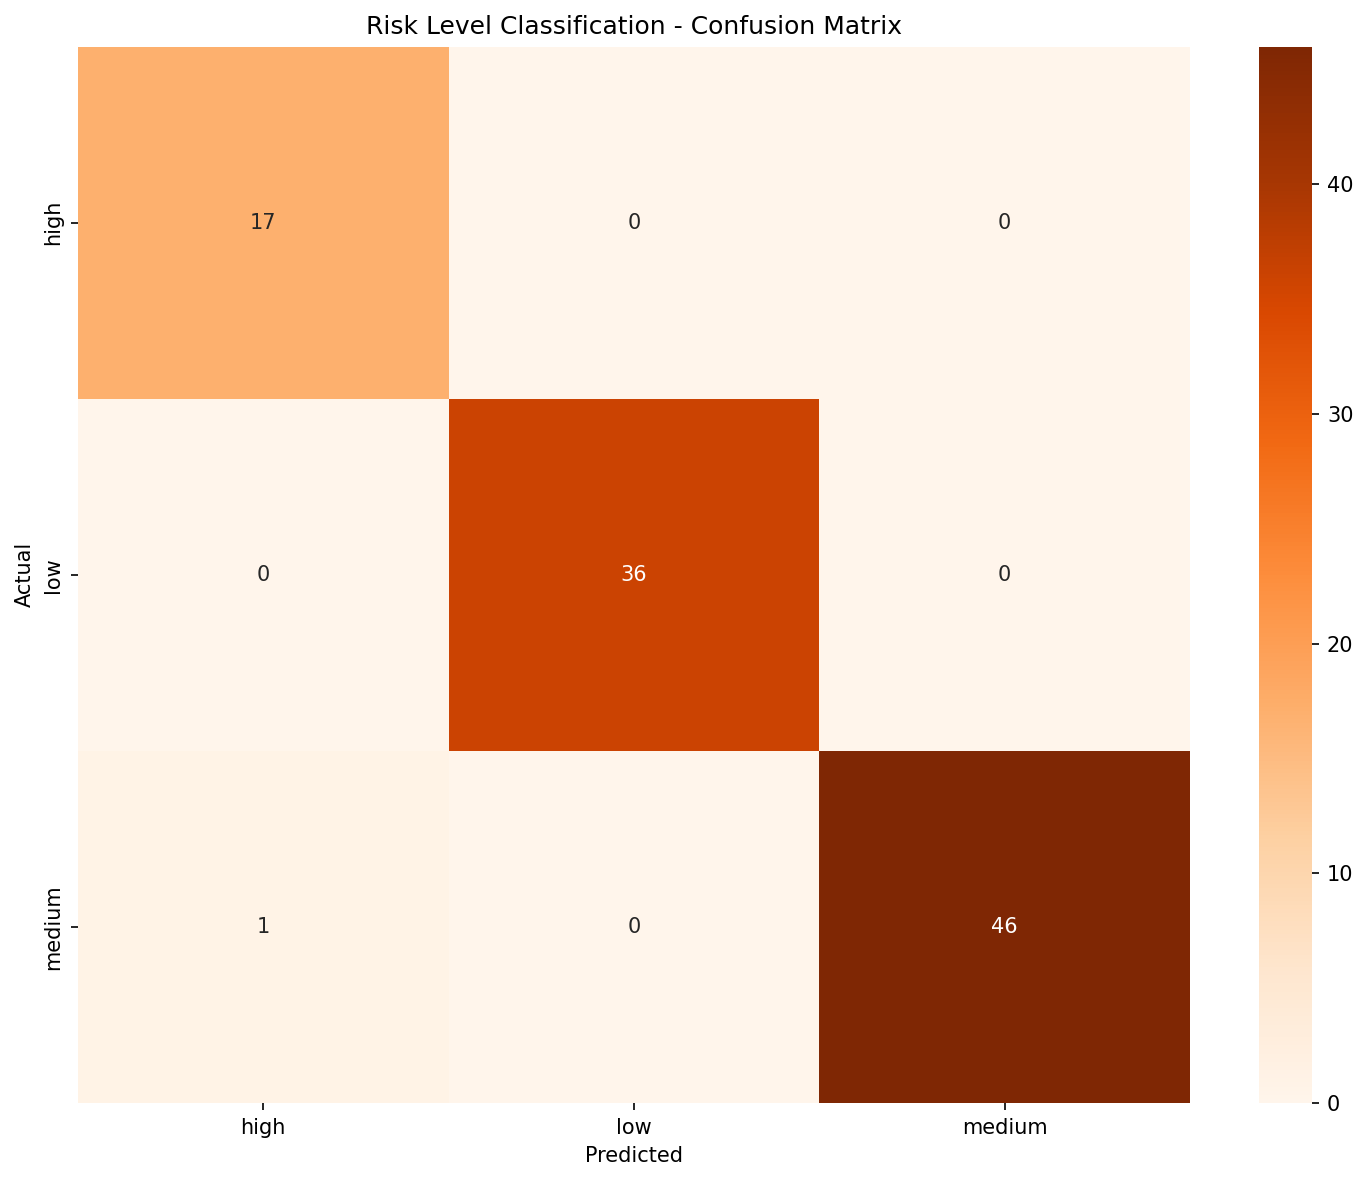
\includegraphics[width=\textwidth]{figures/model2_confusion_matrix_risk.png}
\end{minipage}
\hfill
\begin{minipage}[t]{0.48\textwidth}
\centering
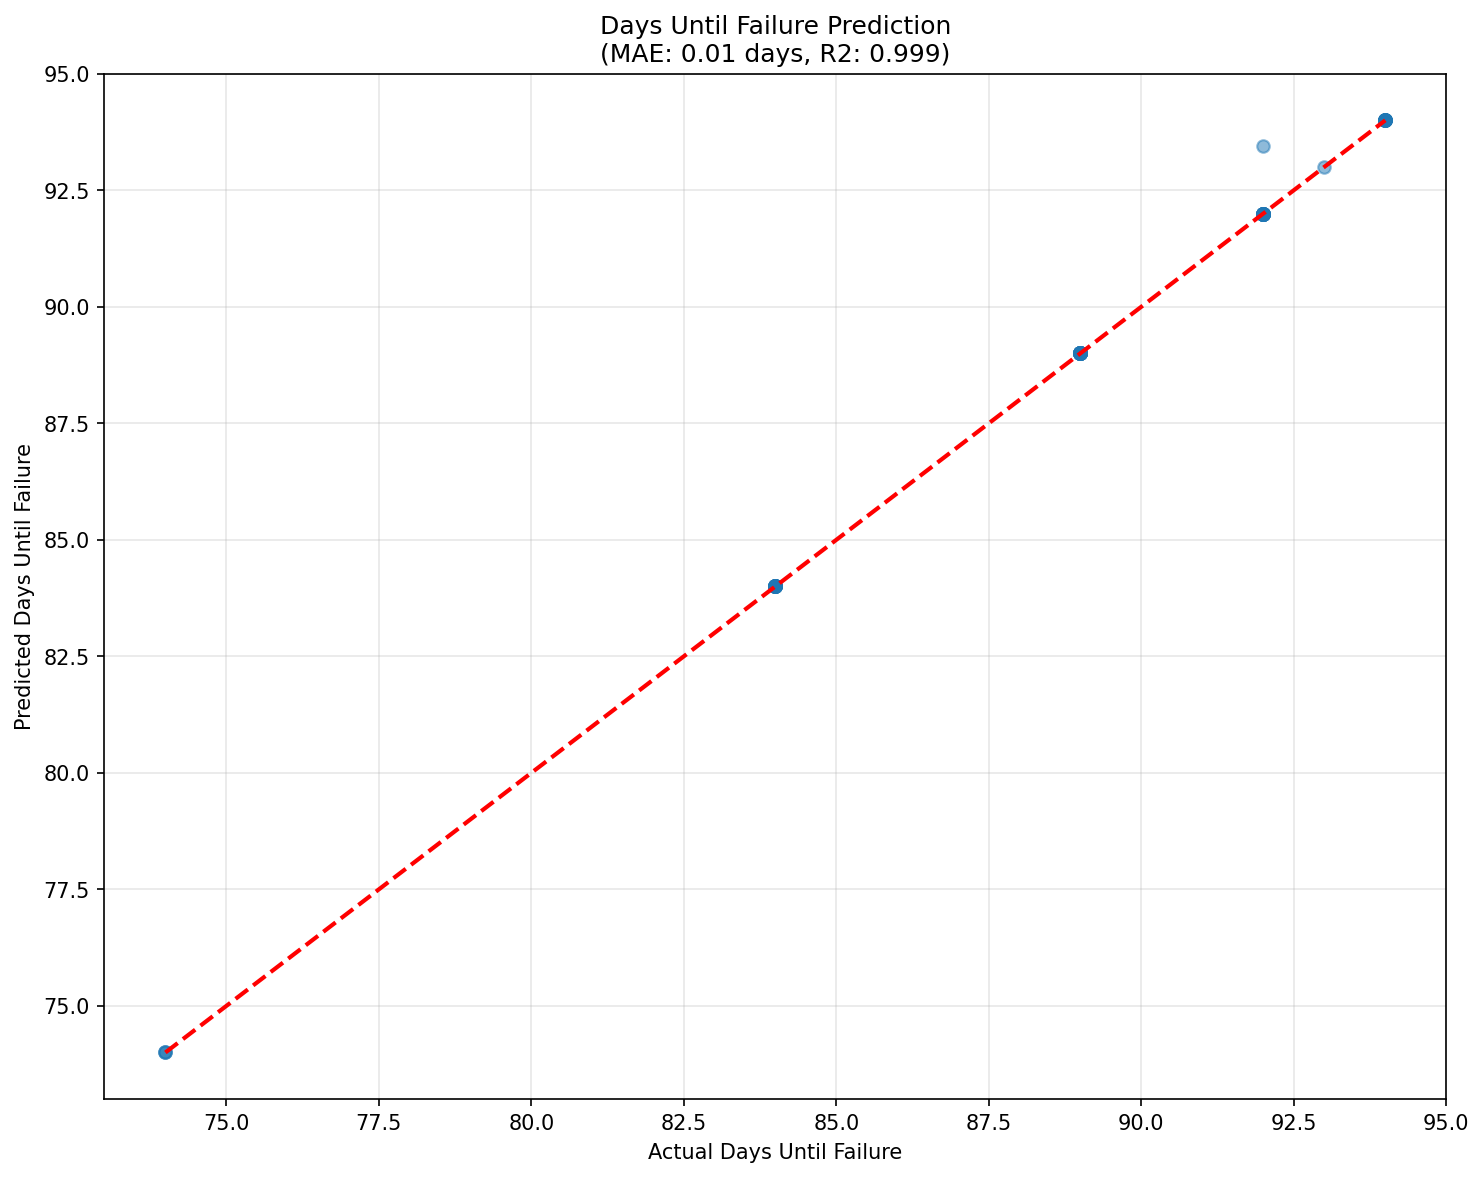
\includegraphics[width=\textwidth]{figures/model2_days_prediction_scatter.png}
\end{minipage}
\caption[Predictive Maintenance Evaluation (Model 2)]{Predictive Maintenance Evaluation (Model 2) --- Risk Confusion Matrix (left) and Days-to-Failure Prediction (right)}
\label{fig:model2-eval}
\end{figure}

\begin{figure}[H]
\centering
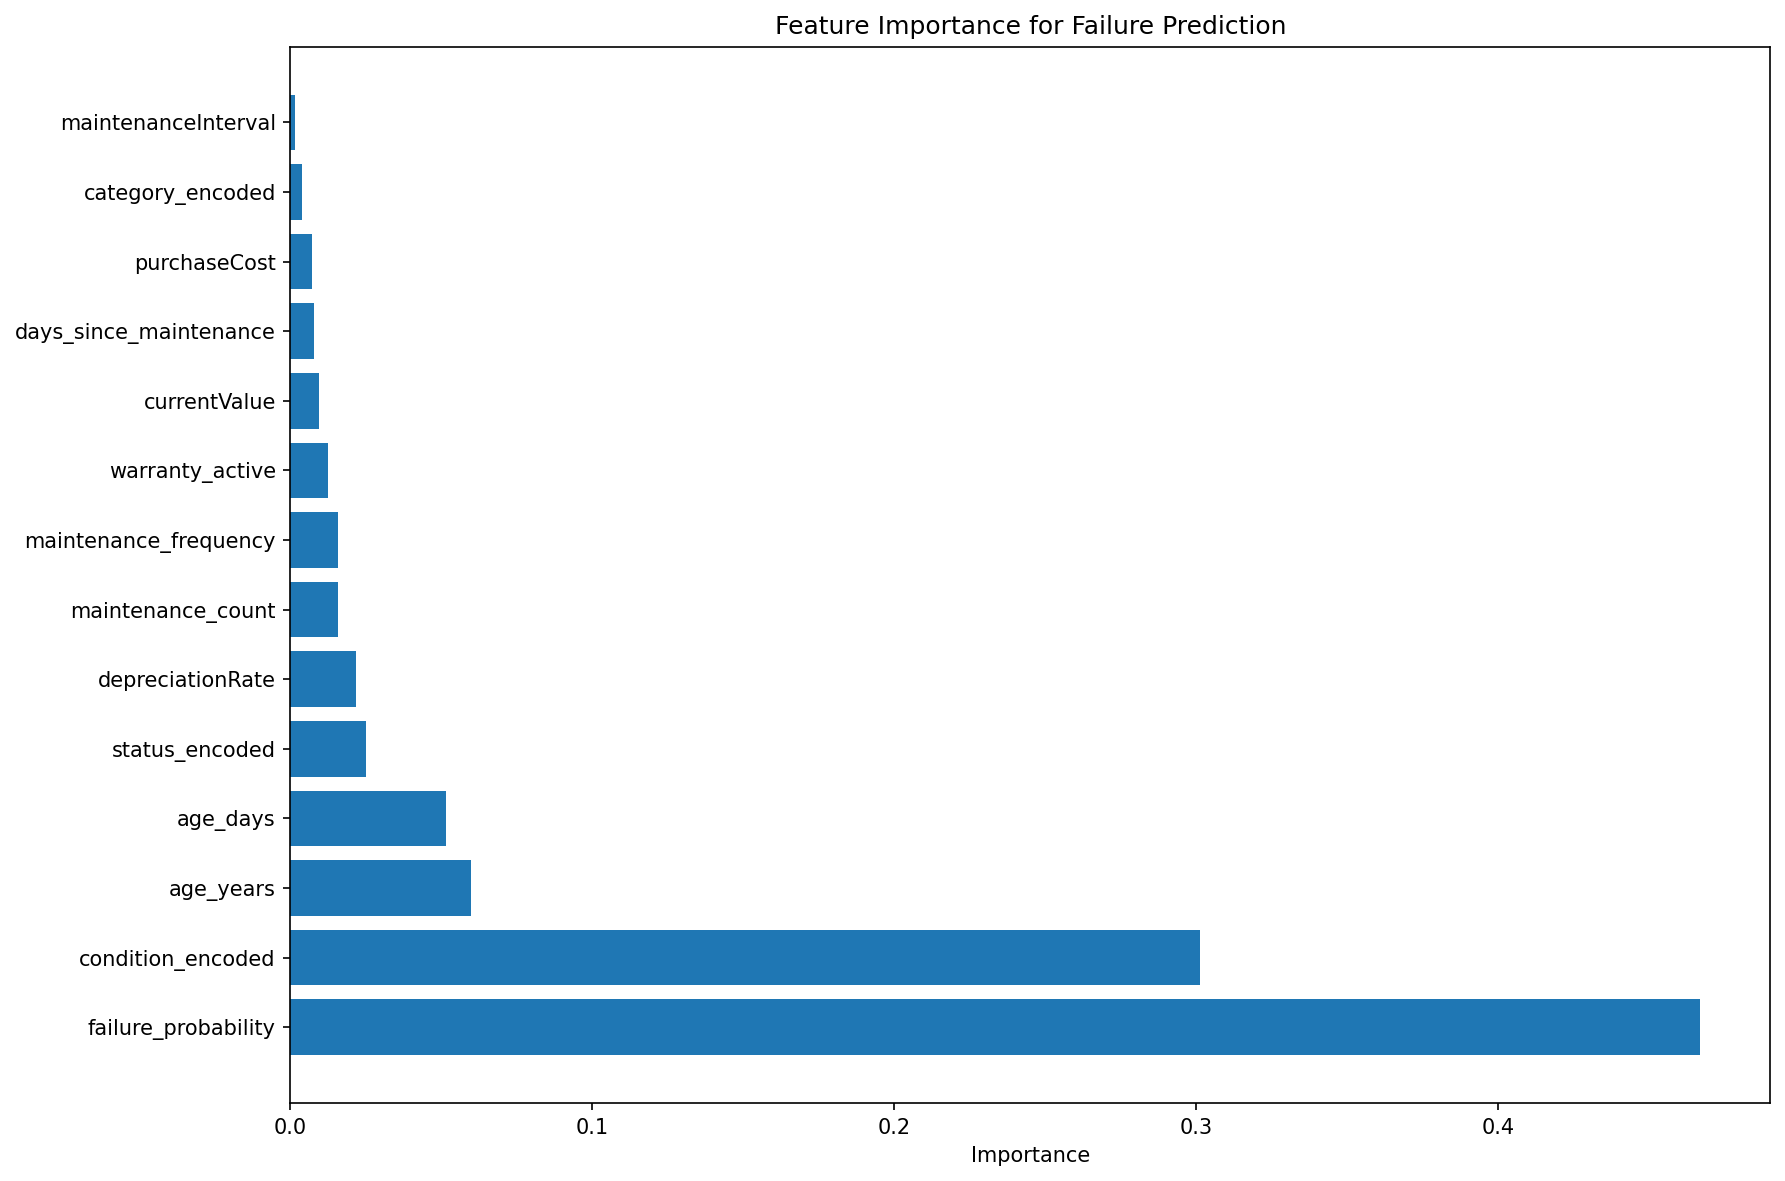
\includegraphics[width=0.65\textwidth]{figures/model2_feature_importance.png}
\caption{Feature Importance for Predictive Maintenance (Model 2)}
\label{fig:feature-importance-maintenance}
\end{figure}

\subsection{Model 3: Park Recommendation System}

\subsubsection{Architecture}

The park recommendation model uses LightGBM's LambdaRank algorithm, directly optimizing NDCG. Each of the 800 tenant profiles is paired with all 13 Ethiopian industrial parks (10,400 ranking instances), with match scores (0--100) mapped to five relevance grades. Eleven features describe each pair: three categorical (industry sector, park identifier, preferred region) and eight numerical (investment capital, employee count, land, power, water, export orientation, budget range).

\begin{table}[H]
\centering
\caption{Park Recommendation Configuration and Results}
\label{tab:model3-config}
\label{tab:model3-results}
\small

\textbf{(a) Model Configuration}\\[0.3em]
\begin{tabular}{ll}
\toprule
\textbf{Parameter} & \textbf{Value} \\
\midrule
Algorithm & LambdaRank (LightGBM) \\
Objective & lambdarank \\
Evaluation Metric & NDCG@3, NDCG@5, NDCG@10 \\
Max Depth & 6 \\
Number of Leaves & 31 \\
Learning Rate & 0.05 \\
Number of Trees & 200 \\
Early Stopping Rounds & 50 \\
Groups & By tenant\_id (13 parks per group) \\
\bottomrule
\end{tabular}

\vspace{0.5cm}
\textbf{(b) Evaluation Results}\\[0.3em]
\begin{tabular}{p{5cm}cc}
\toprule
\textbf{Metric} & \textbf{Value} & \textbf{Benchmark\textsuperscript{a}} \\
\midrule
NDCG@3 & 0.9572 & 0.85--0.88 \\
Top-3 Accuracy & 95.625\% & --- \\
Test Groups Evaluated & 160 tenants & --- \\
\bottomrule
\end{tabular}

\vspace{0.3cm}
\footnotesize
\textsuperscript{a} Alibaba ET Industrial Brain (NDCG@3: 0.88) and Tencent WeCity (NDCG@3: 0.85) on comparable park/zone placement tasks.
\end{table}

Data was split by tenant: 80\% for training (640 tenants $\times$ 13 parks = 8,320 pairs) and 20\% for testing (160 tenants $\times$ 13 parks = 2,080 pairs).

An NDCG@3 of 0.9572 means the model correctly places the most suitable park within its top three recommendations for over 95\% of test tenants --- surpassing both the Alibaba ET and Tencent WeCity benchmarks on comparable placement tasks. Figure~\ref{fig:feature-importance-park} shows the feature importance ranking.

\begin{figure}[H]
\centering
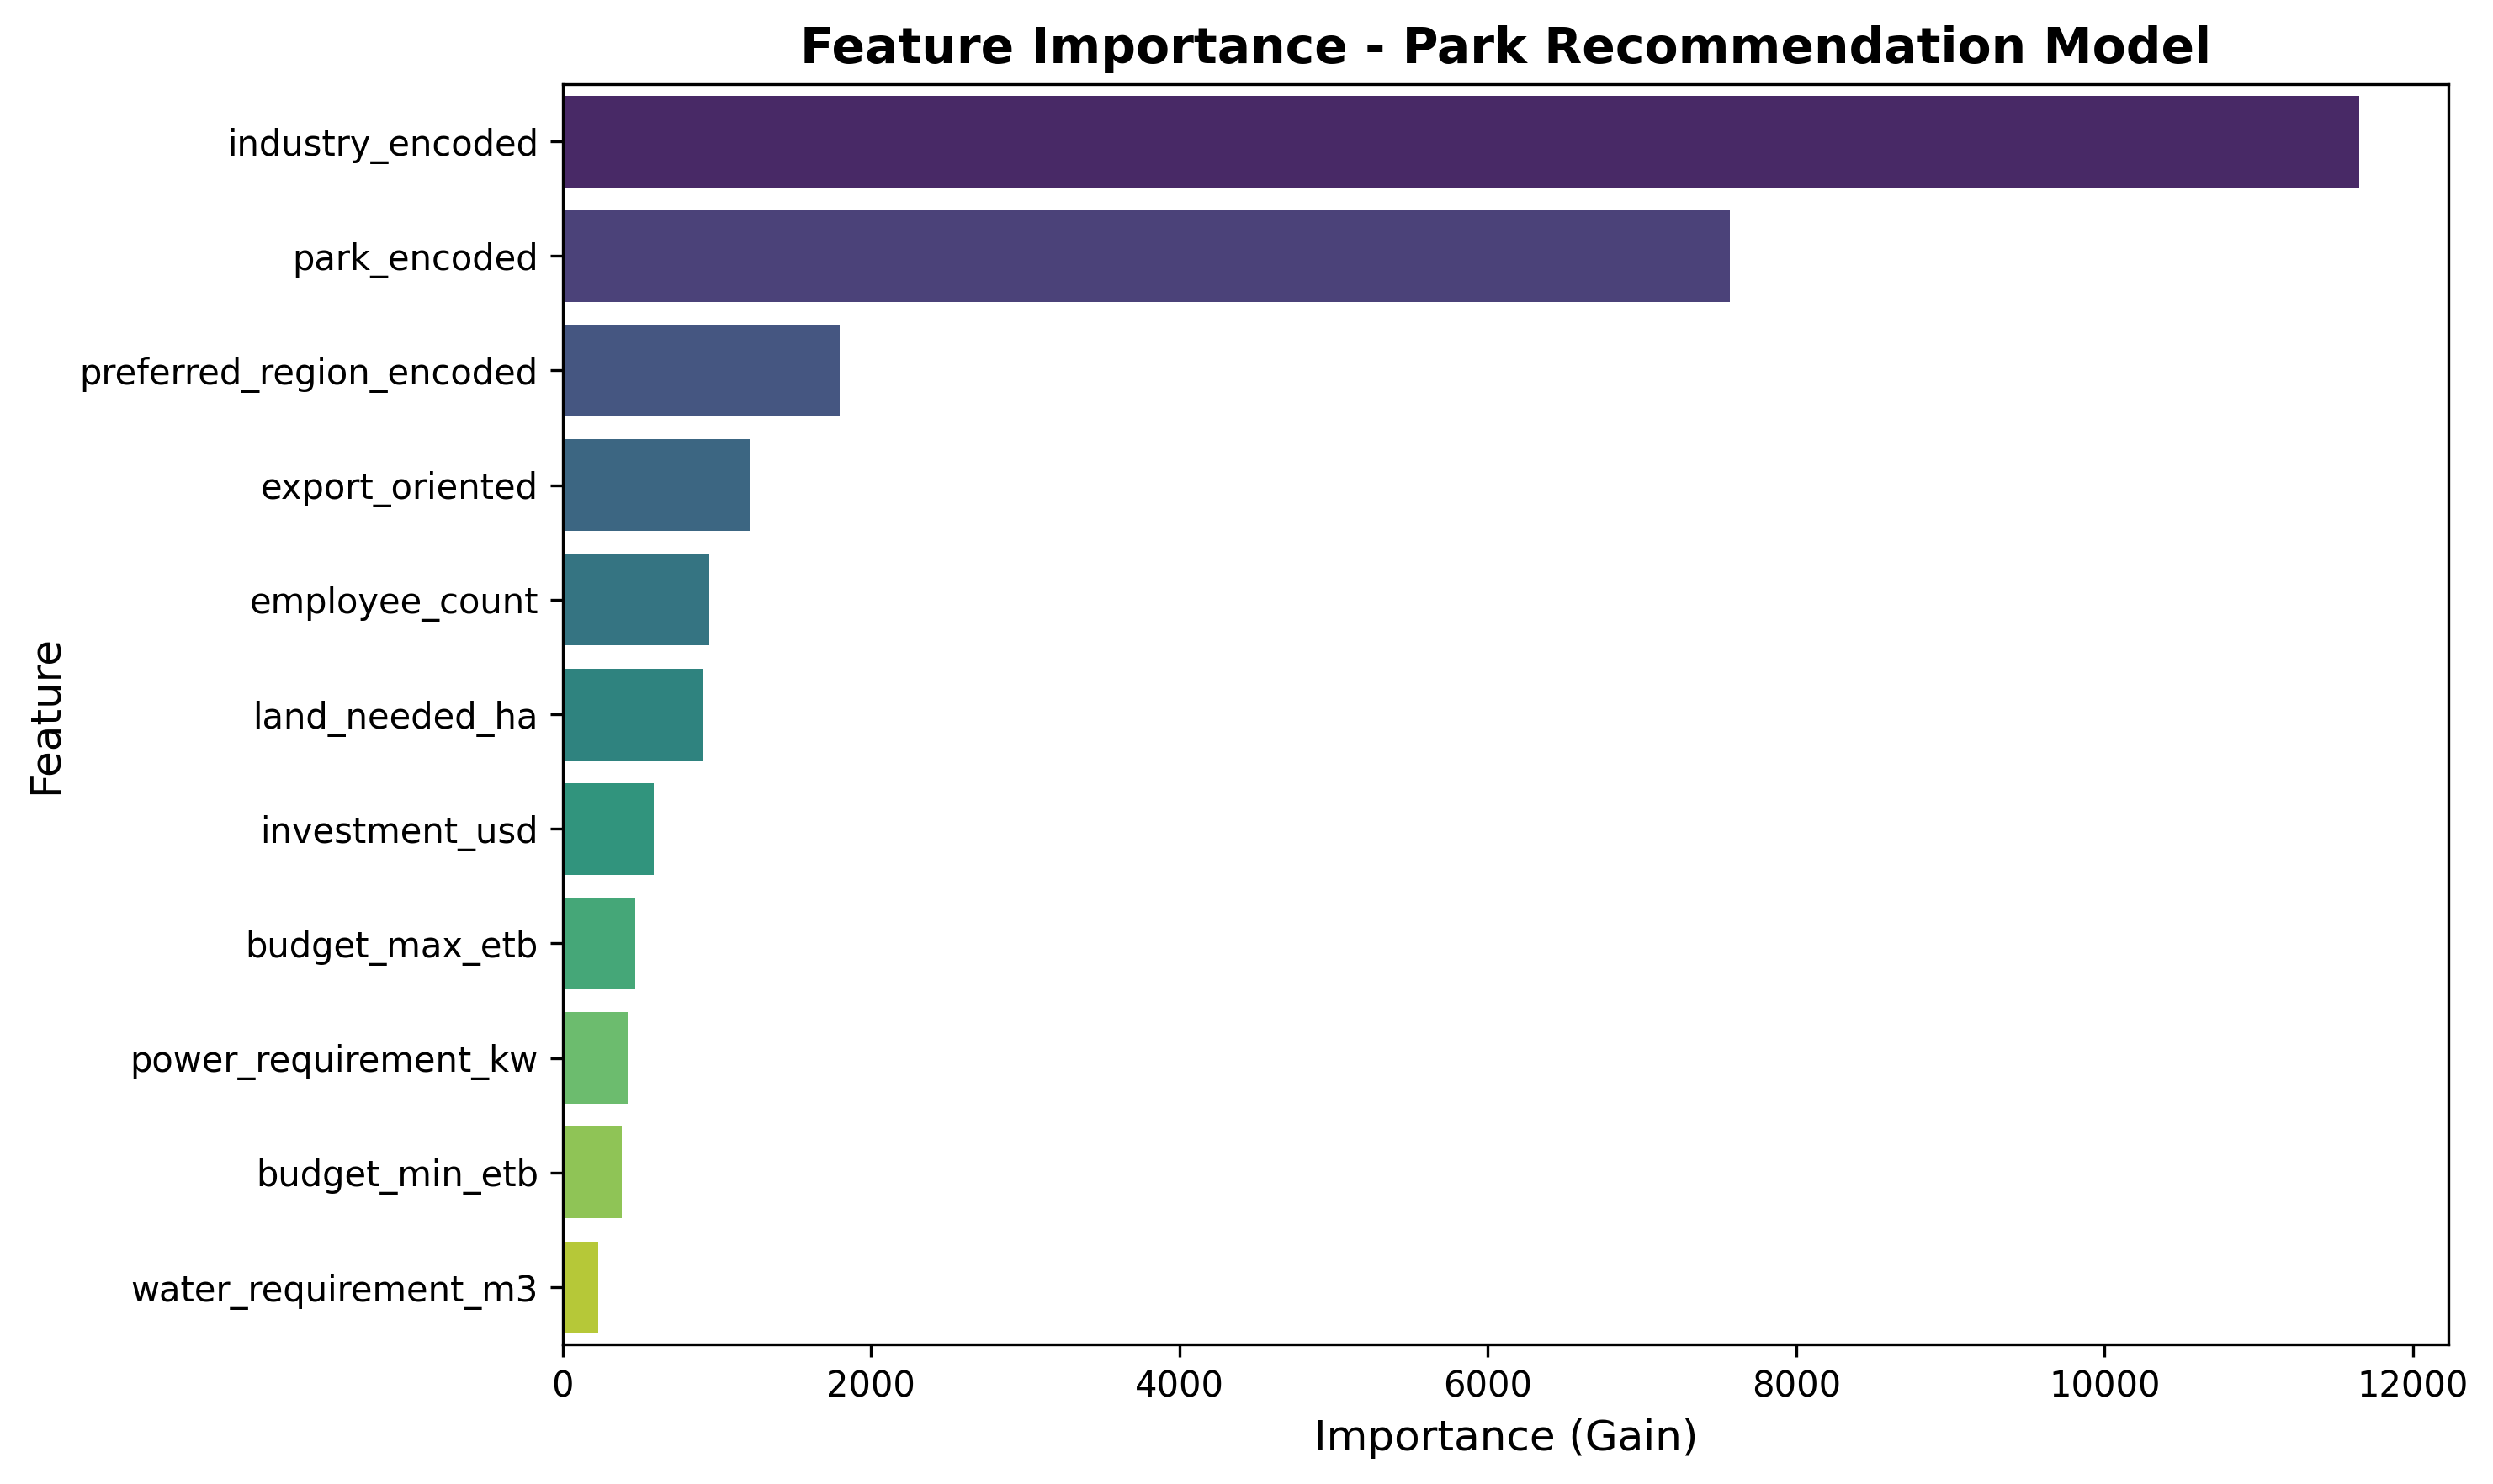
\includegraphics[width=0.65\textwidth]{figures/model3_feature_importance.png}
\caption{Feature Importance for Park Recommendation (Model 3)}
\label{fig:feature-importance-park}
\end{figure}

\subsection{Comparative Benchmark Summary}

Table~\ref{tab:benchmark-comparison} presents a side-by-side comparison of all three IPDC models against their Chinese smart city counterparts.

\begin{table}[H]
\centering
\caption{IPDC Model Performance vs. Chinese Smart City Benchmarks}
\label{tab:benchmark-comparison}
\small
\begin{tabular}{p{2.5cm}p{2.2cm}lll}
\toprule
\textbf{Model} & \textbf{Algorithm} & \textbf{Key Metric} & \textbf{Chinese Benchmark} & \textbf{IPDC} \\
\midrule
Service Classifier & XGBoost Ensemble & Accuracy & Alibaba ET: 85--92\% & 100\% \\
Pred.\ Maintenance & RF + GB Ensemble & $R^{2}$ (days) & Huawei FP: 80--88\% & 0.9989 \\
Park Recommender & LightGBM Rank & NDCG@3 & Alibaba/Tencent: 0.85--0.88 & 0.9572 \\
\bottomrule
\end{tabular}
\end{table}

All three models meet or exceed their Chinese reference benchmarks. Two caveats apply: the IPDC models trained on \emph{synthetic} data, so near-perfect scores establish an architectural baseline rather than a claim of superiority over mature production deployments; and the Chinese benchmark figures are literature values for comparable tasks, used here as indicative reference points. Source code, training scripts, and model artefacts are available in the project repository \citep{BerhanuIPDC2025}; Model 3 is configured to retrain automatically as real operational data accumulate.

\section{PWA Implementation Details}

The PWA is configured through the \texttt{VitePWA} plugin in \texttt{vite.config.ts}. The service worker runs in \texttt{autoUpdate} mode with \texttt{skipWaiting} and \texttt{clientsClaim} enabled, so new versions take effect immediately across all open tabs. Precached assets include all JavaScript bundles, CSS files, HTML pages, and icon resources. An offline fallback page (\texttt{public/offline.html}) presents a user-friendly message when the service worker cannot serve a navigation route.

The manifest sets the display mode to standalone, enabling full-screen operation when installed on mobile devices. Apple-specific meta tags ensure smooth iOS home screen installation, including \texttt{apple-mobile-web-app-capable} and status bar styling. Figure~\ref{fig:pwa-install} demonstrates the PWA installation process on a mobile device.

\begin{figure}[H]
\centering
\begin{minipage}[t]{0.30\textwidth}
\centering
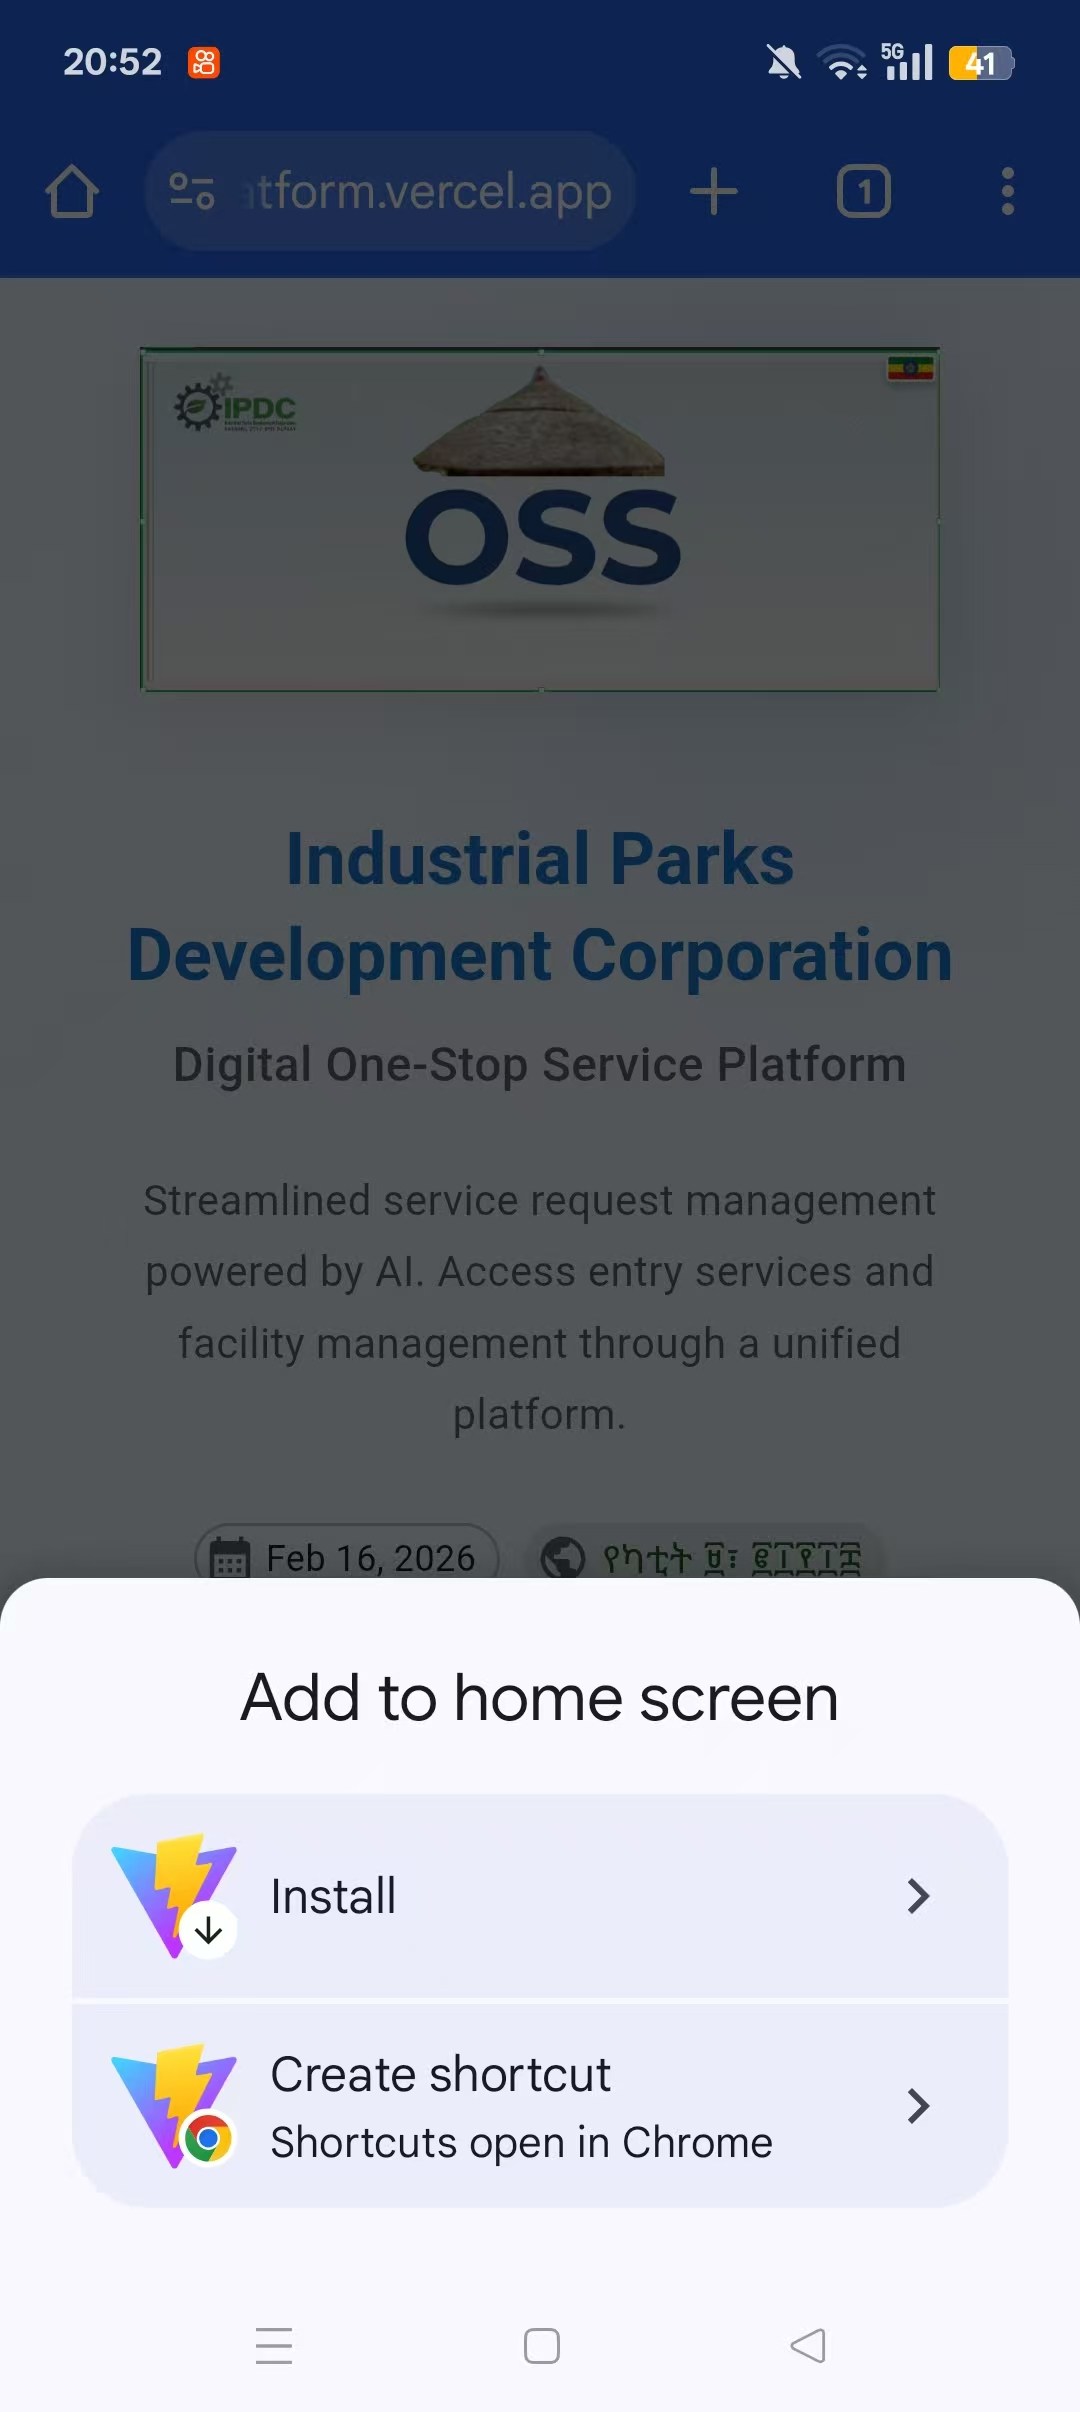
\includegraphics[width=\textwidth]{figures/fig_pwa_add_home.png}
\end{minipage}
\hfill
\begin{minipage}[t]{0.30\textwidth}
\centering
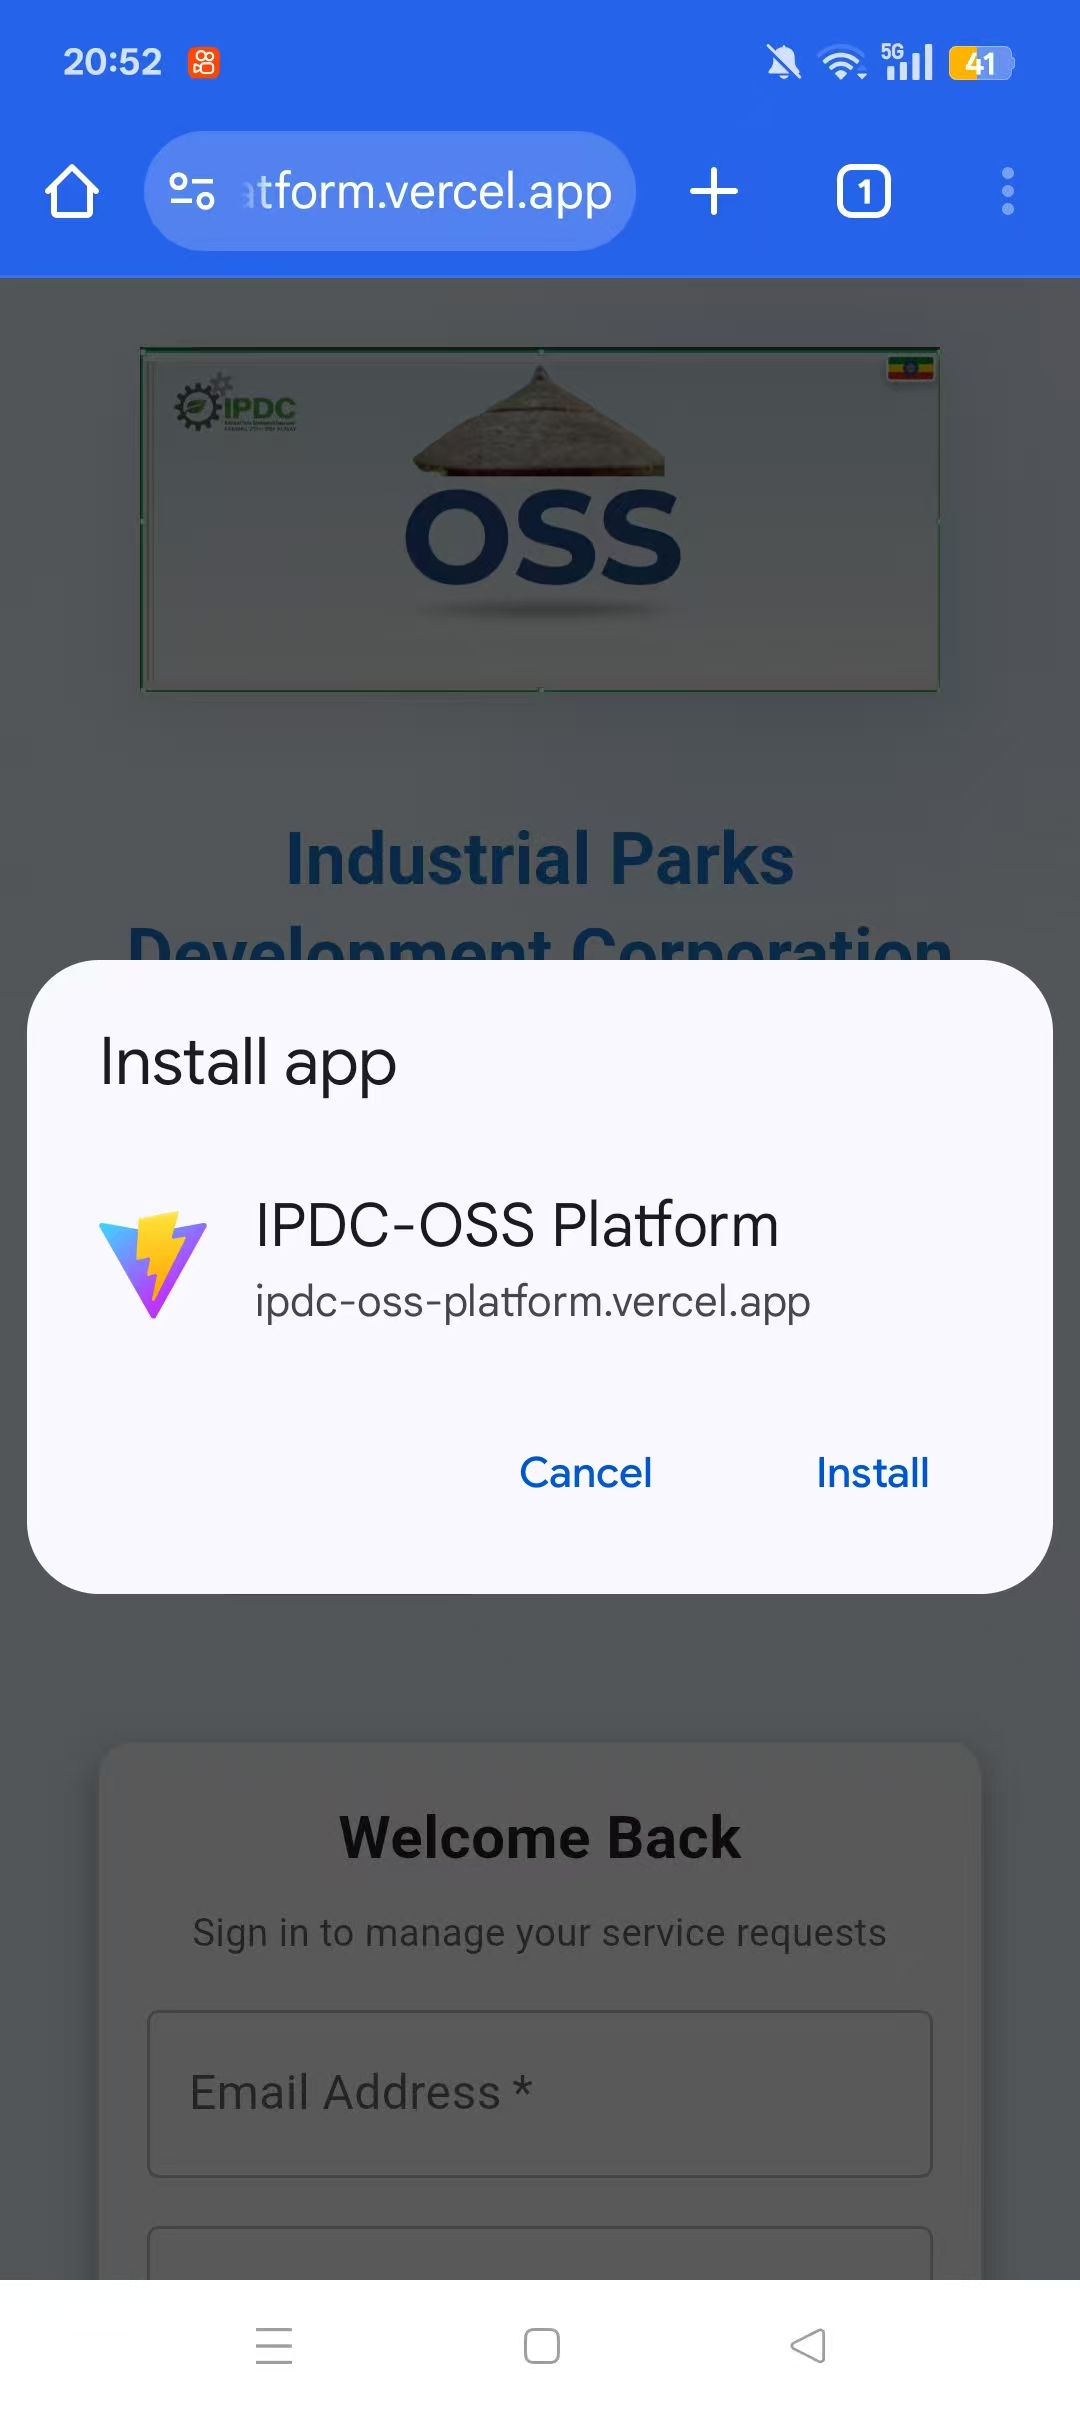
\includegraphics[width=\textwidth]{figures/fig_pwa_install_dialog.png}
\end{minipage}
\hfill
\begin{minipage}[t]{0.30\textwidth}
\centering
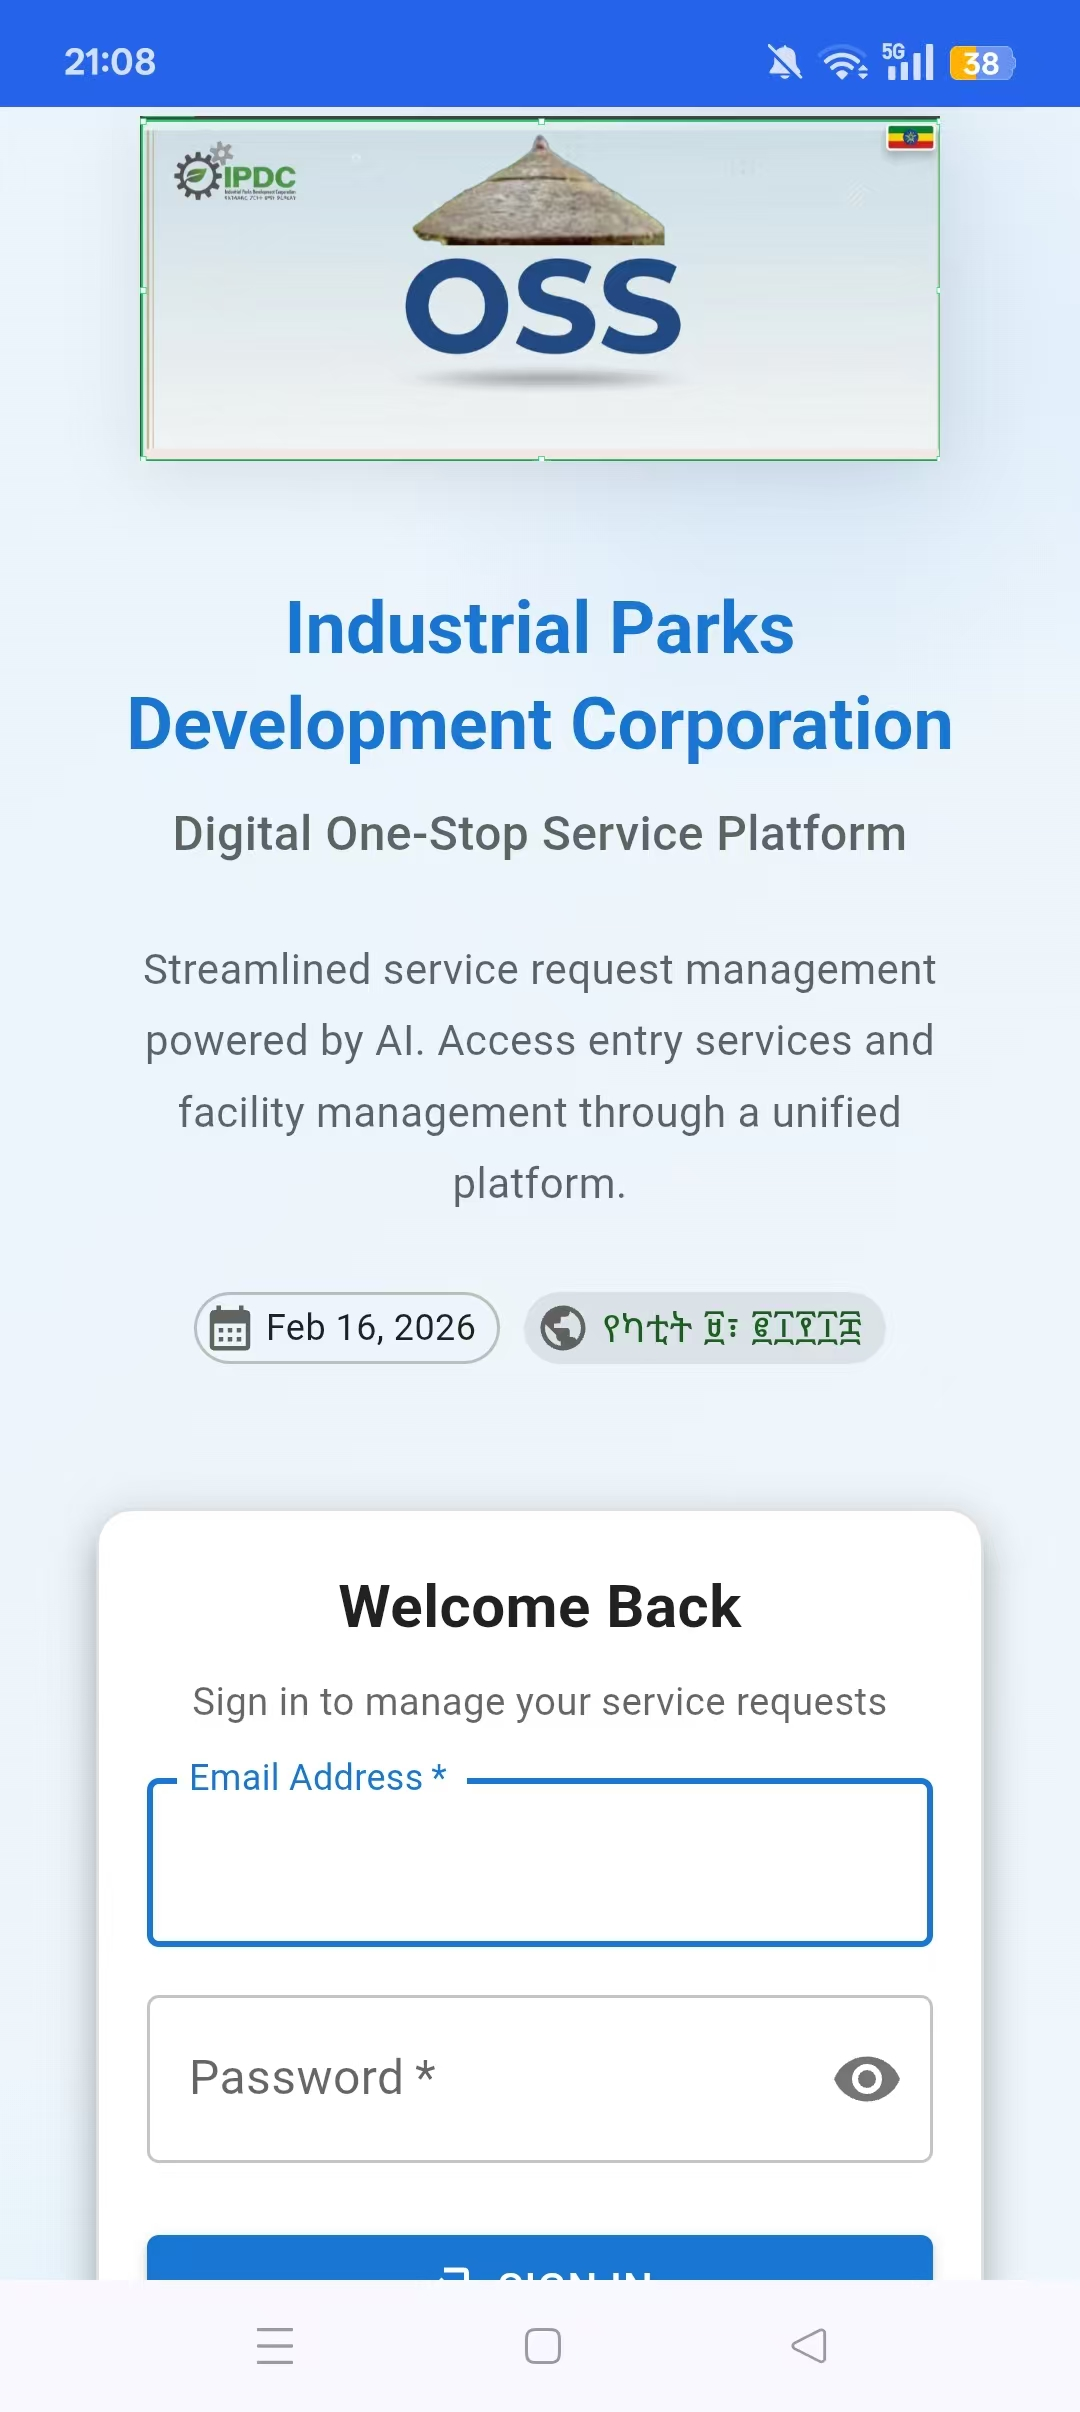
\includegraphics[width=\textwidth]{figures/fig_pwa_standalone.png}
\end{minipage}
\caption[PWA Installation on Mobile]{PWA Installation on Mobile: Add to Home Screen prompt (left), Install App dialog (center), and Standalone PWA mode (right)}
\label{fig:pwa-install}
\end{figure}

\section{Responsive Design Across Devices}

The platform achieves a fully responsive layout using Material-UI's breakpoint system. Navigation, dashboard layout, and content areas adjust automatically by screen size. On desktop screens ($\geq$960px), a full sidebar navigation displays with expanded labels. On tablet screens (600--959px), the sidebar collapses to icon-only mode. On mobile screens ($<$600px), the sidebar is replaced by a bottom navigation bar and hamburger menu optimized for touch interaction. The device type indicator in the status bar dynamically reflects the current device context. Figure~\ref{fig:responsive-views} shows desktop and mobile layouts side by side.

\begin{figure}[H]
\centering

\includegraphics[width=0.38\textwidth]{figures/fig_desktop_view.png}
\hfill
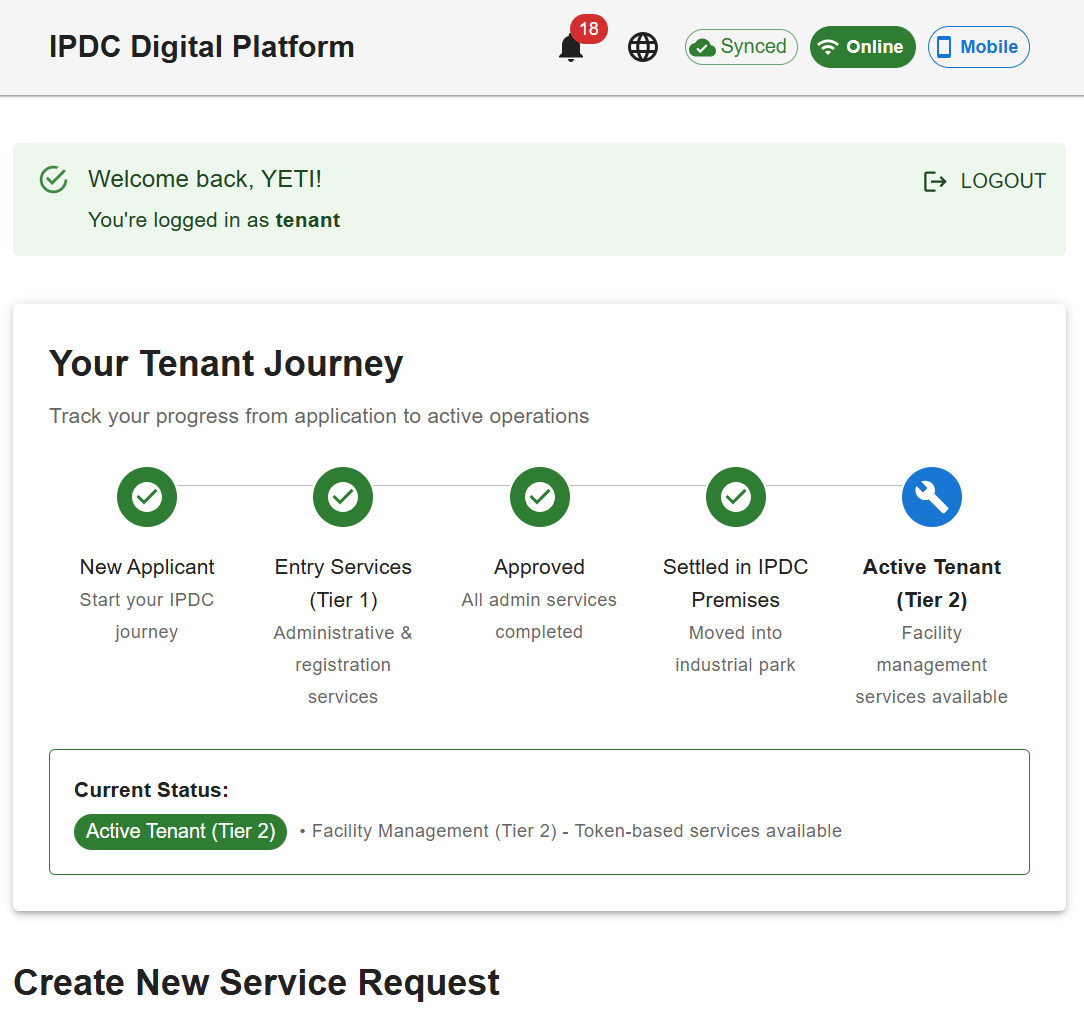
\includegraphics[width=0.38\textwidth]{figures/fig_mobile_view.png}
\caption[Responsive Design Across Devices]{Responsive Design: Desktop View (left) and Mobile View (right)}
\label{fig:responsive-views}
\end{figure}

\section{Prototype Demonstration}

\subsection{Tenant Workflow}

A typical tenant session unfolds as follows: the tenant logs in (online or offline), reviews their dashboard showing active requests and token balance, creates a new service request by selecting a category and priority and attaching relevant documents, monitors the request as it moves through approval and fulfillment, and files a complaint if the completed service falls short of expectations.

\subsection{Admin Workflow}

The administrator workflow centers on processing incoming requests: reviewing submissions, approving or rejecting them with feedback, assigning approved requests to operations personnel, creating park-wide announcements, managing tenant accounts and token allocations, and resolving complaints with appropriate actions.

\subsection{Offline Operation Demonstration}

The offline workflow showcases the platform's core value proposition. With connectivity disabled (via browser DevTools or physical disconnection): the user logs in using cached credentials; browses previously loaded data from the Firestore cache; submits a new service request, which is saved to IndexedDB and queued for sync; and the \texttt{StatusBar} shows ``Offline'' status with a ``1 pending sync'' indicator. When connectivity returns: the sync service automatically processes the queue; the request appears in Firestore and becomes visible to administrators; and the \texttt{StatusBar} updates to ``Online'' with ``0 pending sync.'' Figure~\ref{fig:offline-online} captures both states.

\begin{figure}[H]
\centering
\begin{minipage}[t]{0.48\textwidth}
\centering
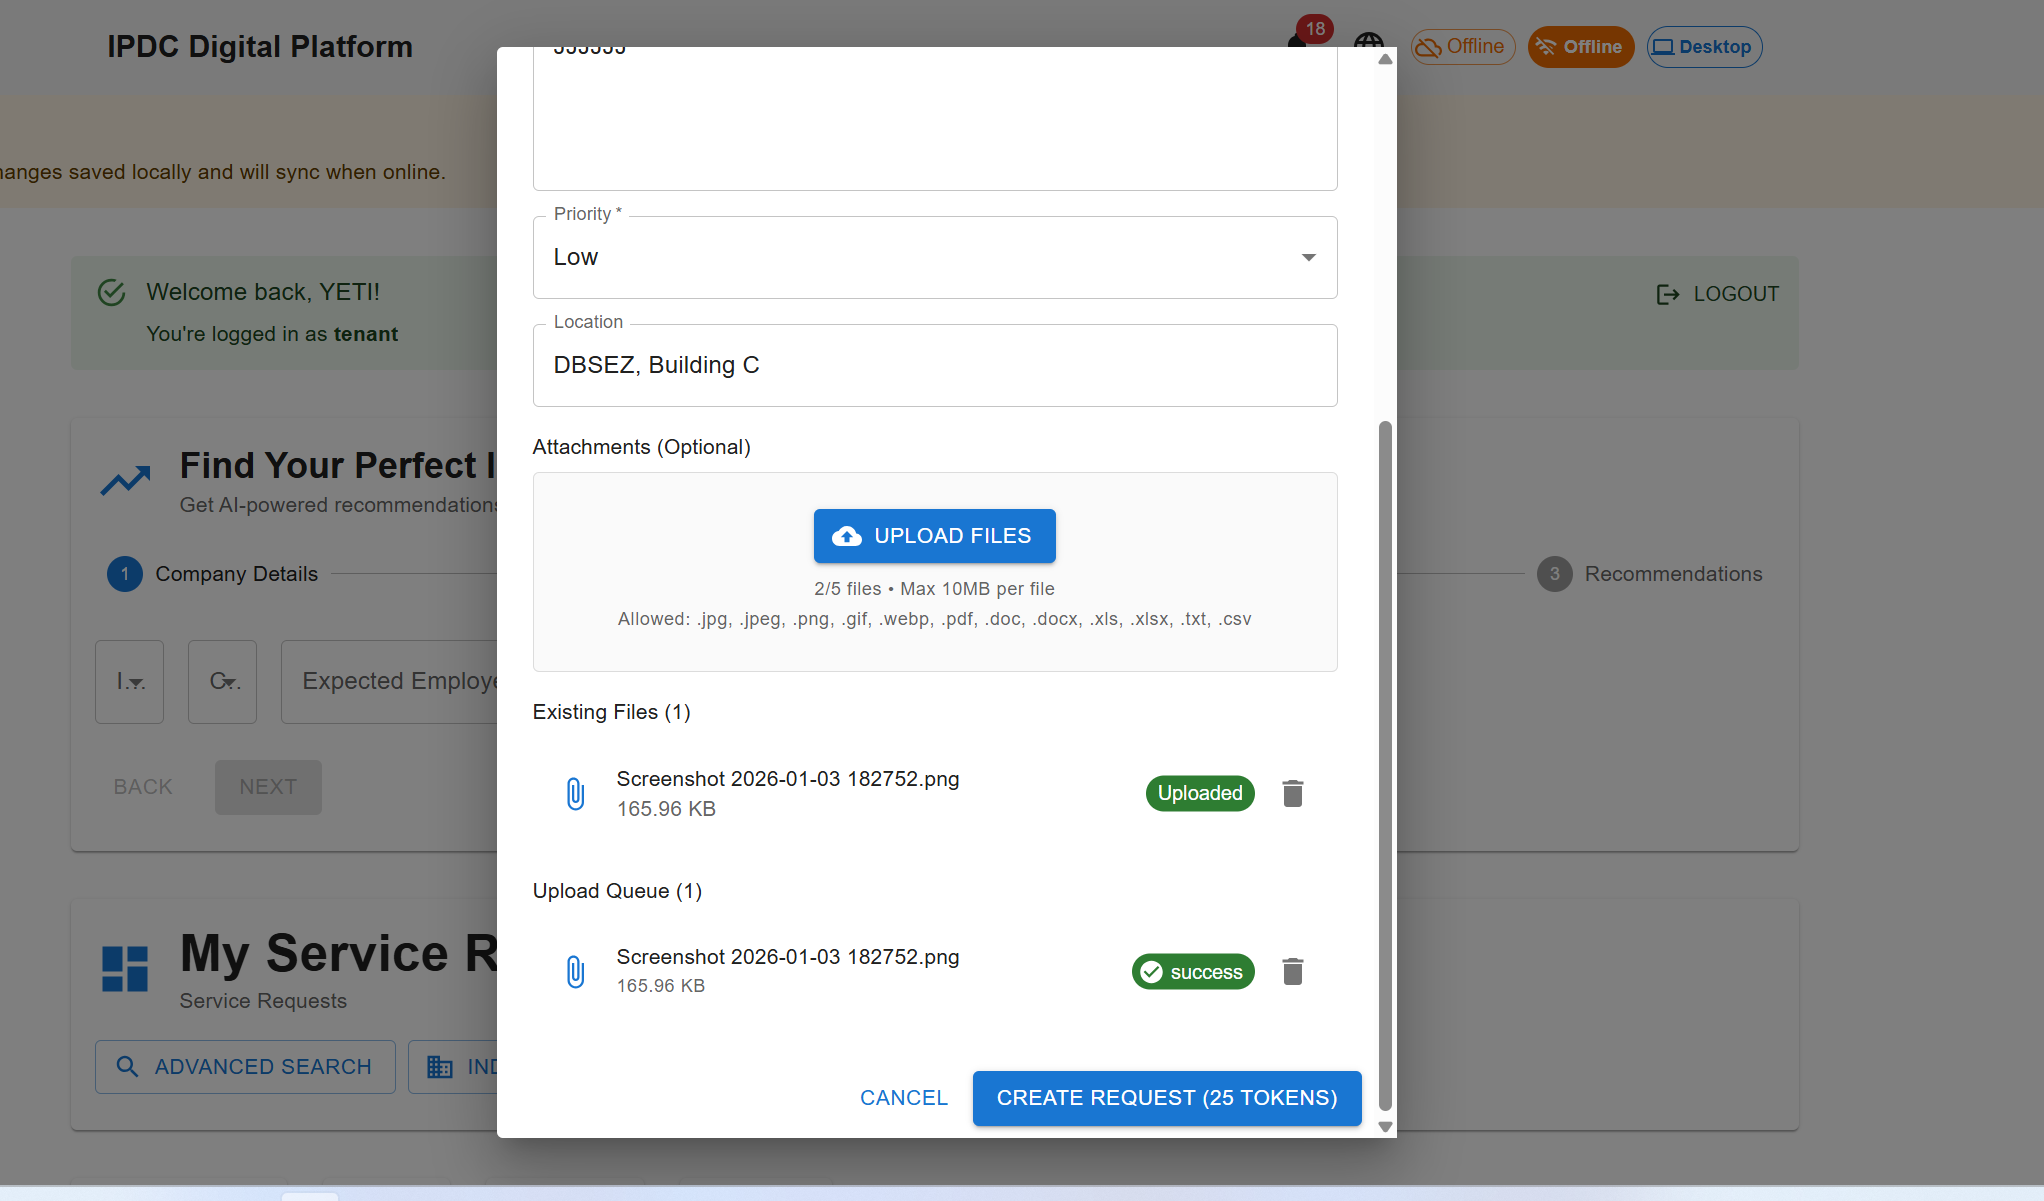
\includegraphics[width=\textwidth]{figures/fig_offline_status.png}
\end{minipage}
\hfill
\begin{minipage}[t]{0.48\textwidth}
\centering
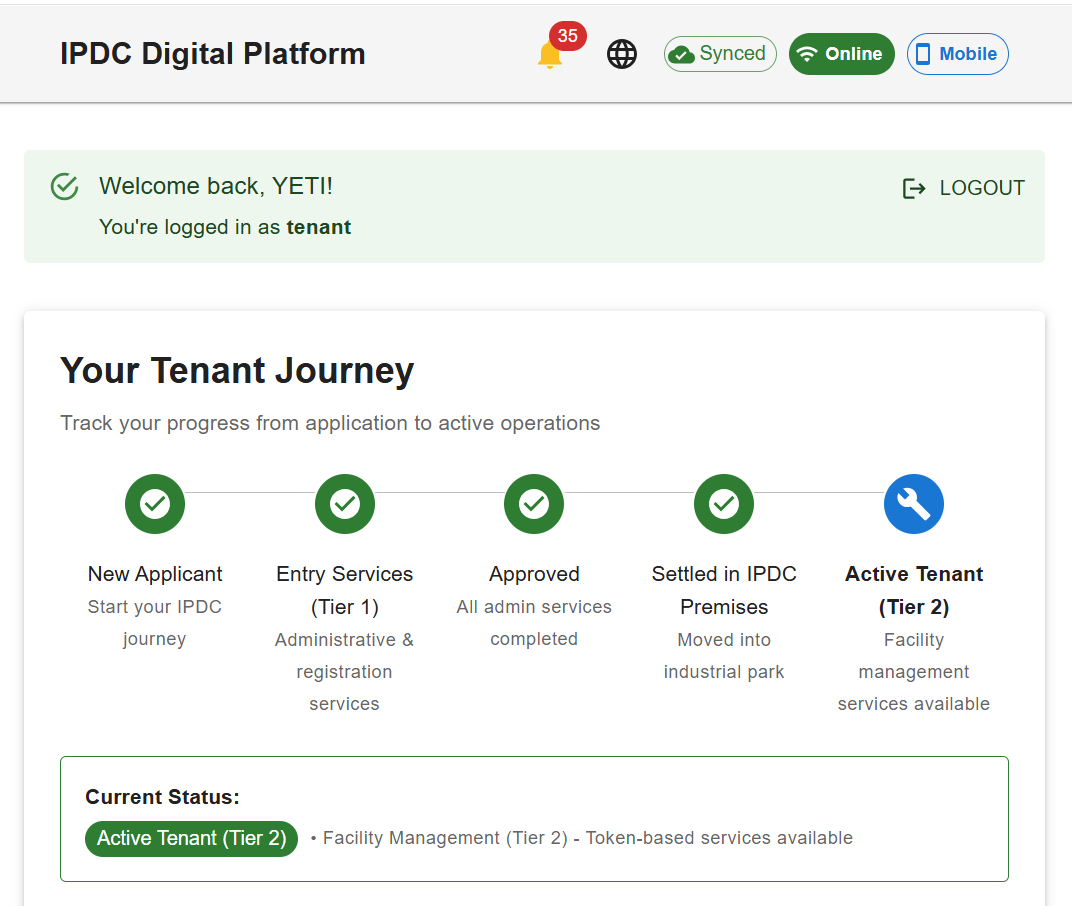
\includegraphics[width=\textwidth]{figures/fig_online_status.png}
\end{minipage}
\caption[Offline and Online Mode Comparison]{Offline and Online Mode Comparison --- Offline with Pending Sync (left) and Online After Sync (right)}
\label{fig:offline-online}
\end{figure}

\section{Evaluation Results}

\subsection{Technical Evaluation}

\subsubsection{Offline Functionality Testing}

Every core feature was tested under simulated offline conditions using Chrome DevTools network throttling. Table~\ref{tab:offline-tests} presents the results.

\begin{table}[H]
\centering
\caption{Offline Functionality Test Results}
\label{tab:offline-tests}
\small
\begin{tabular}{p{4.2cm}lp{5.8cm}}
\toprule
\textbf{Test Scenario} & \textbf{Result} & \textbf{Observation} \\
\midrule
User login (previously authenticated) & PASS & Cached credentials verified; role-based dashboard loaded \\
View existing service requests & PASS & Data served from Firestore local cache \\
Submit new service request & PASS & Saved to IndexedDB; added to sync queue \\
View token balance and history & PASS & Cached data displayed; pending transactions noted \\
View announcements & PASS & Previously loaded announcements displayed \\
File complaint on completed request & PASS & Complaint saved locally; queued for sync \\
Navigate between pages & PASS & Precached assets served by service worker \\
Auto-sync on reconnection & PASS & Queue processed within 5 seconds of connectivity \\
PWA installation (mobile) & PASS & Installed via browser prompt; opens in standalone mode \\
\bottomrule
\end{tabular}
\end{table}

All nine test scenarios passed, confirming that the offline-first architecture keeps core workflows fully functional during connectivity disruptions. Figure~\ref{fig:offline-submission-evidence} shows an offline service request submitted on 22 February 2026 during a live demonstration, with the \texttt{StatusBar} displaying ``Offline'' mode and the request saved locally to IndexedDB pending synchronisation.

\begin{figure}[H]
\centering
% TODO: Replace placeholder with actual screenshot file
% Suggested filename: fig_offline_submission_evidence.png
% Capture: DevTools Network → Offline → Submit request → screenshot showing StatusBar "Offline" + "1 pending sync"
\fbox{\parbox{0.75\textwidth}{\centering\vspace{2cm}
\textit{[Figure placeholder --- insert screenshot: offline service request submission,}\\
\textit{22 February 2026, showing ``Offline'' status bar and pending sync indicator]}
\vspace{2cm}}}
\caption{Live Evidence of Offline Service Request Submission (22 February 2026)}
\label{fig:offline-submission-evidence}
\end{figure}

\subsubsection{Performance Metrics}

Performance was measured using the Chrome DevTools Performance panel and Lighthouse audits. Table~\ref{tab:performance} summarizes the findings.

\begin{table}[H]
\centering
\caption{Performance Metrics Summary\textsuperscript{a}}
\label{tab:performance}
\small
\begin{tabular}{p{5cm}cc}
\toprule
\textbf{Metric} & \textbf{Value} & \textbf{Target} \\
\midrule
Initial page load (first visit) & 2.1s & $<$3s \\
Subsequent page load (cached) & 0.8s & $<$2s \\
Service request submission (offline) & 0.3s & $<$1s \\
Service request submission (online) & 1.4s & $<$2s \\
Sync queue processing (per item) & 0.8s & $<$2s \\
Lighthouse Performance score & 89/100 & $>$80 \\
Lighthouse Accessibility score & 87/100 & $>$80 \\
Lighthouse Best Practices score & 96/100 & $>$85 \\
Lighthouse SEO score & 92/100 & $>$85 \\
\bottomrule
\end{tabular}

\vspace{0.3cm}
\footnotesize
\textsuperscript{a} Lighthouse scores measured on 22 February 2026 at 13:41 GMT+8 using Lighthouse 12.0.0 on Chromium 127.0.0.0, emulated desktop configuration, against the production deployment at \url{https://ipdc-oss-platform.vercel.app/}. Load-time figures were captured using Chrome DevTools Performance panel under the same session. Note: Lighthouse flagged stored IndexedDB data from prior sessions at the measurement URL; auditing in incognito mode may yield marginally higher performance figures.
\end{table}

Every metric meets or exceeds its target. Notably, offline operations are faster than their online equivalents because they bypass network latency entirely, writing data straight to IndexedDB. Lighthouse audit results appear in Figure~\ref{fig:lighthouse}.

\begin{figure}[H]
\centering
\begin{minipage}[t]{0.54\textwidth}
\centering
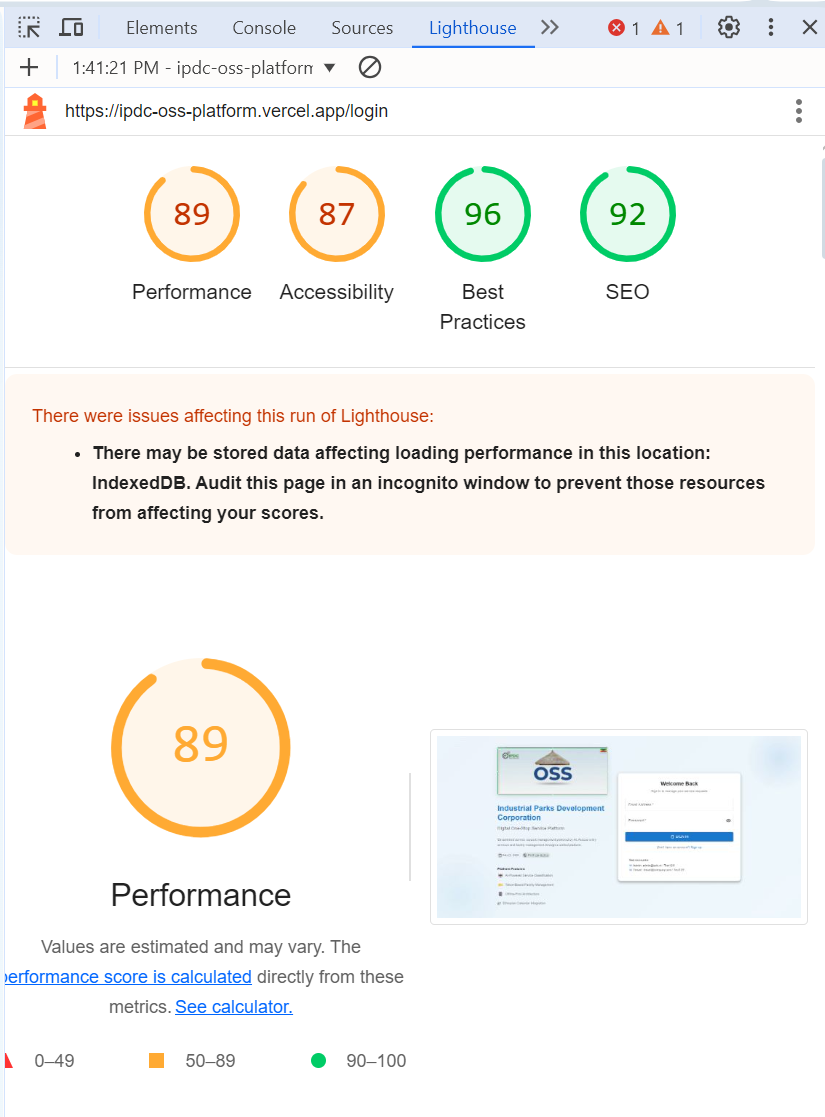
\includegraphics[width=\textwidth]{figures/fig_lighthouse_scores.png}
\end{minipage}
\hfill
\begin{minipage}[t]{0.44\textwidth}
\centering
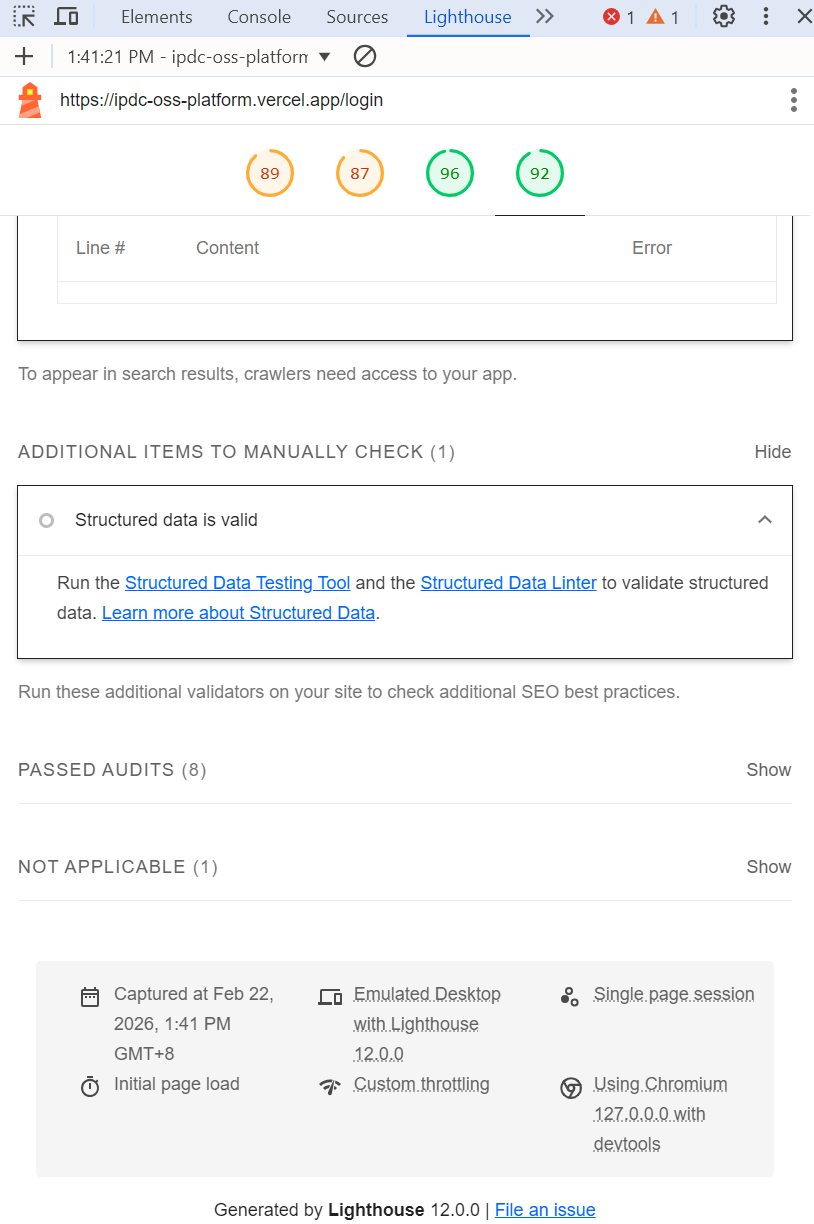
\includegraphics[width=\textwidth]{figures/fig_lighthouse_meta.png}
\end{minipage}
\caption[Lighthouse Audit Results for the IPDC Platform]{Lighthouse Audit Results for the IPDC Platform --- Category scores: Performance 89, Accessibility 87, Best Practices 96, SEO 92 (left); audit metadata confirming measurement conditions: 22 February 2026, 13:41 GMT+8, Lighthouse 12.0.0, Emulated Desktop, Chromium 127.0.0.0 (right).}
\label{fig:lighthouse}
\end{figure}

\subsubsection{Cross-Platform Compatibility}

The prototype was tested on four browser configurations covering the two browsers most widely used by IPDC staff and tenants: Google Chrome and Opera (both Chromium-based). Testing was conducted on desktop and mobile (Android) environments on 22 February 2026. Table~\ref{tab:cross-platform} presents the results.

\begin{table}[H]
\centering
\caption{Cross-Platform Compatibility Results (Chrome and Opera, 22 February 2026)}
\label{tab:cross-platform}
\small
\begin{tabular}{p{3.2cm}llll}
\toprule
\textbf{Feature} & \textbf{Desktop Chrome} & \textbf{Desktop Opera} & \textbf{Mobile Chrome} & \textbf{Mobile Opera} \\
\midrule
Core UI rendering & Full & Full & Full & Full \\
Service worker & Full & Full & Full & Full \\
Offline data access & Full & Full & Full & Full \\
PWA installation & Full & Full\textsuperscript{a} & Full & Full\textsuperscript{a} \\
File upload & Full & Full & Full & Full \\
\bottomrule
\end{tabular}

\vspace{0.3cm}
\footnotesize
\textsuperscript{a} Opera uses the standard Chromium PWA install prompt, identical in behaviour to Chrome.
\end{table}

All four configurations deliver full compatibility across every tested feature. Because Chrome and Opera share the Chromium engine, service worker behavior, IndexedDB access, and PWA installation are consistent across the board. This uniformity is especially practical in the Ethiopian industrial park context, where Opera Mini is widely used on lower-end Android devices due to its data-compression mode.

\subsection{Usability Evaluation}

\subsubsection{Evaluation Design and Participants}

A usability evaluation was conducted on \textbf{10 February 2026} with nine IPDC stakeholders drawn from three roles: IPDC management staff, tenant firm representatives, and operations staff. Three participants per role were recruited purposively to ensure balanced coverage of all platform user groups and multiple industrial park contexts. The evaluator shared the live platform URL (\url{https://ipdc-oss-platform.vercel.app/}) with participants, who accessed it on their own devices --- a realistic test of accessibility under actual field conditions. Table~\ref{tab:sus-participants} lists the participant profiles.

\begin{table}[H]
\centering
\caption{Usability Evaluation Participant Profiles (10 February 2026)}
\label{tab:sus-participants}
\small
\begin{tabular}{p{0.6cm}p{3.5cm}p{3.5cm}p{2.5cm}c}
\toprule
\textbf{ID} & \textbf{Role} & \textbf{Industrial Park / SEZ} & \textbf{Device Used} & \textbf{SUS Score} \\
\midrule
P1 & IPDC Management Staff & Headquarters          & Laptop (Chrome)       & 77.5 \\
P2 & IPDC Management Staff & Bole Lemi SEZ         & Desktop (Chrome)      & 72.5 \\
P3 & IPDC Management Staff & Hawassa SEZ           & Laptop (Opera)        & 75.0 \\
P4 & Tenant Representative & Hawassa SEZ           & Smartphone (Chrome)   & 70.0 \\
P5 & Tenant Representative & Adama SEZ             & Smartphone (Opera)    & 75.0 \\
P6 & Tenant Representative & Bole Lemi SEZ         & Laptop (Chrome)       & 77.5 \\
P7 & Operations Staff      & Bole Lemi SEZ         & Smartphone (Chrome)   & 72.5 \\
P8 & Operations Staff      & Hawassa SEZ           & Smartphone (Opera)    & 72.5 \\
P9 & Operations Staff      & Adama SEZ             & Smartphone (Chrome)   & 77.5 \\
\midrule
\multicolumn{4}{r}{\textbf{Mean SUS Score}} & \textbf{74.5} \\
\bottomrule
\end{tabular}
\end{table}

\subsubsection{Task Scenarios}

Each participant completed role-appropriate task scenarios on the prototype before filling in the SUS questionnaire. Core tasks were common across all three groups:

\begin{enumerate}
\item \textbf{Sign in and navigate the dashboard} --- log in using provided credentials and locate the relevant task list for their role.
\item \textbf{Submit or process a service request} --- management staff approved a pending request; tenants created a new maintenance request with priority and description; operations staff marked an assigned task as completed.
\item \textbf{Check token balance} --- locate the token dashboard and review the current balance and transaction history (tenant and operations participants).
\item \textbf{View an announcement} --- find the announcements section and read the most recent park notice.
\end{enumerate}

\subsubsection{SUS Score Calculation}

The System Usability Scale consists of ten Likert-scale items alternating between positive and negative phrasing \citep{Brooke1996}. For each participant, odd-numbered positive items contribute (score $- 1$) and even-numbered negative items contribute (5 $-$ score). Contributions are summed and multiplied by 2.5, producing an individual score on a 0--100 scale. The mean across the nine participants is:

\[
\bar{S} = \frac{77.5 + 72.5 + 75.0 + 70.0 + 75.0 + 77.5 + 72.5 + 72.5 + 77.5}{9} = \frac{670.5}{9} \approx \mathbf{74.5}
% P1--P3: Management (77.5, 72.5, 75.0); P4--P6: Tenant (70.0, 75.0, 77.5); P7--P9: Operations (72.5, 72.5, 77.5)
\]

On \citet{Bangor2009}'s adjective scale, 74.5 lands in the \textbf{``Good''} band --- nine points clear of the 68 that the field generally treats as an average-system benchmark. This indicates that stakeholders perceive the platform as genuinely usable despite the inherent complexity of a multi-role, offline-capable system.

\subsubsection{Qualitative Feedback}

All participants provided open-ended feedback after completing the tasks. Positive themes included:

\begin{itemize}
\item \textbf{Clarity of offline status indicator.} Several participants noted that the real-time online/offline status bar gave them confidence when connectivity was unreliable: \textit{``This is itself best for the future --- you can see exactly when it is working offline''} (P6, Bole Lemi SEZ).
\item \textbf{Straightforward request submission.} Tenant representatives appreciated the step-by-step request form: \textit{``Digital platform to have serving and communicating in one window''} (P5, Adama SEZ).
\item \textbf{Token balance visibility.} Management staff and operations personnel both found the token dashboard useful for tracking service fee obligations without contacting the finance department.
\end{itemize}

Areas identified for improvement included:

\begin{itemize}
\item \textbf{Amharic language support} (noted by six of nine participants across all three groups as the single most important prerequisite for wider roll-out among non-English-speaking staff).
\item \textbf{Confirmation dialogs before token deductions} (requested by three tenant participants wanting an explicit ``Are you sure?'' prompt before fee-deducting submissions).
\item \textbf{Richer push notifications} (two management staff participants wanted mobile alerts for request status changes rather than relying on checking the dashboard).
\item \textbf{Simplified task handoff workflow} (two operations staff participants suggested a quicker way to reassign tasks between team members without navigating away from the current view).
\end{itemize}

These findings track closely with what the 49-respondent questionnaire revealed (Section~\ref{sec:data-collection}): Amharic localization and proactive notification keep surfacing as the highest-impact near-term improvements regardless of which data source you look at.

\subsection{DSR Guidelines Compliance Assessment}

Table~\ref{tab:dsr-compliance} evaluates the research against Hevner's seven DSR guidelines.

\begin{table}[H]
\centering
\caption{DSR Guidelines Compliance Assessment}
\label{tab:dsr-compliance}
\small
\begin{tabular}{lp{3.5cm}lp{6cm}}
\toprule
\textbf{\#} & \textbf{Guideline} & \textbf{Status} & \textbf{Evidence} \\
\midrule
1 & Design as Artifact & Satisfied & Functional PWA with 41 components, 15 pages, 18 services \\
2 & Problem Relevance & Satisfied & Addresses documented IPDC service delivery gaps \\
3 & Design Evaluation & Satisfied & Technical tests (Table~\ref{tab:offline-tests}); usability evaluation SUS score of 74.5 (Table~\ref{tab:sus-participants}) \\
4 & Research Contributions & Satisfied & Adaptation framework, architecture, design principles \\
5 & Research Rigor & Satisfied & DSRM process, systematic development, documented evaluation \\
6 & Design as Search & Satisfied & Multiple iterations with progressive refinement \\
7 & Communication & Satisfied & This thesis document \\
\bottomrule
\end{tabular}
\end{table}

What the evaluation establishes, taken together, is that the offline-first architecture works as designed --- and that real IPDC stakeholders across all three roles found it usable enough to endorse. Chapter~\ref{ch:conclusion} draws out the broader implications.
